\section{client}
È il package che racchiude tutte le parti del front-end. Contiene le componenti che vengono eseguite nel browser da un qualsiasi utente, fornendo loro un’interfaccia grafica per interagire con il sistema.\begin{center}
		\begin{figure}[H]
			\centering \includegraphics[scale=4, max width=\textwidth, max height=\myheight]{../img/diagrammiClassi/client.png}
			\caption{Diagramma package - client}
		\end{figure}
	\end{center}\subsection{client::view}
È il package che contiene tutte le classi che costituiscono la view del client. 
Ogni componente si occupa della visualizzazione di una particolare porzione dell'interfaccia di un utente.\begin{center}
		\begin{figure}[H]
			\centering 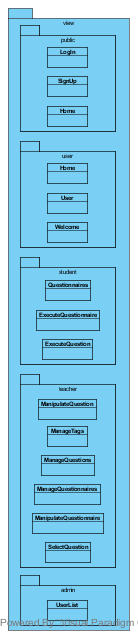
\includegraphics[scale=4, max width=\textwidth, max height=\myheight]{../img/diagrammiClassi/client/view.png}
			\caption{Diagramma package - client::view}
		\end{figure}
	\end{center}\subsubsection{client::view::public}
È il package che contiene tutte le classi che costituiscono la view della porzione publica di client. Ogni componente si occupa della visualizzazione di una particolare porzione dell'interfaccia di un utente non autenticato.\begin{center}
		\begin{figure}[H]
			\centering 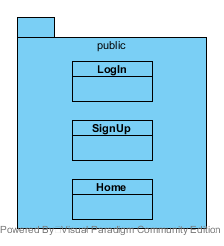
\includegraphics[scale=4, max width=\textwidth, max height=\myheight]{../img/diagrammiClassi/client/view/public.png}
			\caption{Diagramma package - client::view::public}
		\end{figure}
	\end{center}\hypertarget{client::view::public::LogIn}{}
\subsubsubsection[LogIn]{client::view::public::LogIn}
\begin{center}
			\begin{figure}[H]
				\centering 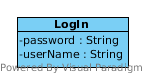
\includegraphics[scale=4, max width=\textwidth, max height=\myheight]{../img/diagrammiClassi/client/view/public/LogIn.png}
				\caption{Diagramma classe - client::view::public::LogIn}
			\end{figure}
		\end{center}\begin{description}
\item[Descrizione] \hfill \\
 La classe che si occupa della visualizzazione dell'area di autenticazione
\item[Attributi] \hfill \\
 \vspace{-7mm}
\begin{itemize}
\item password : String (contiene la password inserita dall'utente )
\item userName : String (contiene l' username inserito dall'utente )
\end{itemize}

\end{description}

\vspace{0.5cm}
\hypertarget{client::view::public::SignUp}{}
\subsubsubsection[SignUp]{client::view::public::SignUp}
\begin{center}
			\begin{figure}[H]
				\centering 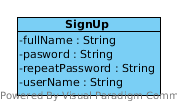
\includegraphics[scale=4, max width=\textwidth, max height=\myheight]{../img/diagrammiClassi/client/view/public/SignUp.png}
				\caption{Diagramma classe - client::view::public::SignUp}
			\end{figure}
		\end{center}\begin{description}
\item[Descrizione] \hfill \\
 La classe che si occupa della visualizzazione sul client dell'area di registrazione
\item[Attributi] \hfill \\
 \vspace{-7mm}
\begin{itemize}
\item fullName : String (contiene il nome completo inserito dall'utente )
\item pasword : String (contiene la password inserita dall'utente )
\item repeatPassword : String (contiene la password inserita per seconda volta dall'utente )
\item userName : String (contiene l'username inserito dall'utente )
\end{itemize}

\end{description}

\vspace{0.5cm}
\subsubsection{client::view::student}
È il package che contiene tutte le classi che costituiscono la view della porzione di client per uno studente. Ogni componente si occupa della visualizzazione di una particolare porzione dell'interfaccia di uno studente.\begin{center}
		\begin{figure}[H]
			\centering 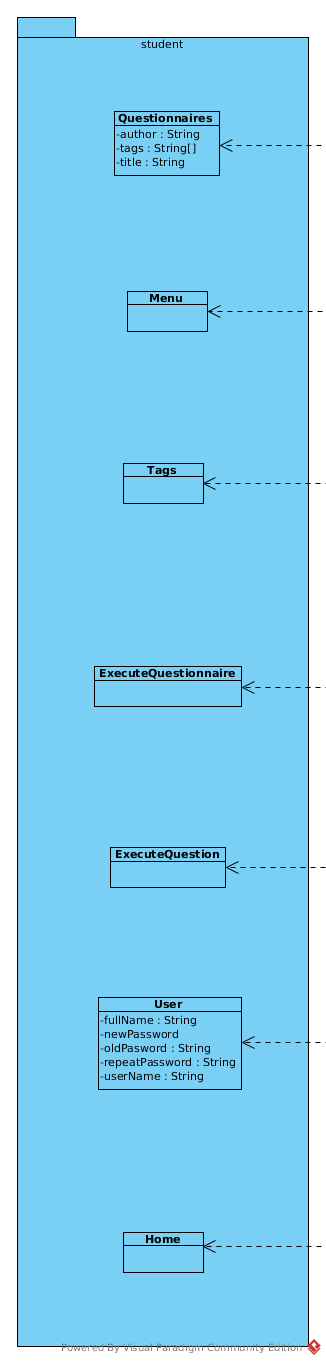
\includegraphics[scale=4, max width=\textwidth, max height=\myheight]{../img/diagrammiClassi/client/view/student.png}
			\caption{Diagramma package - client::view::student}
		\end{figure}
	\end{center}\hypertarget{client::view::student::Menu}{}
\subsubsubsection[Menu]{client::view::student::Menu}
\begin{center}
			\begin{figure}[H]
				\centering 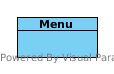
\includegraphics[scale=4, max width=\textwidth, max height=\myheight]{../img/diagrammiClassi/client/view/student/Menu.png}
				\caption{Diagramma classe - client::view::student::Menu}
			\end{figure}
		\end{center}\begin{description}
\item[Descrizione] \hfill \\
 La classe che si occupa della visualizzazione del menu di navigazione per le azioni di uno studente
\end{description}

\vspace{0.5cm}
\hypertarget{client::view::student::Questionnaires}{}
\subsubsubsection[Questionnaires]{client::view::student::Questionnaires}
\begin{center}
			\begin{figure}[H]
				\centering 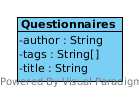
\includegraphics[scale=4, max width=\textwidth, max height=\myheight]{../img/diagrammiClassi/client/view/student/Questionnaires.png}
				\caption{Diagramma classe - client::view::student::Questionnaires}
			\end{figure}
		\end{center}\begin{description}
\item[Descrizione] \hfill \\
 La classe che si occupa della visualizzazione della lista dei questionari eseguibili
\item[Attributi] \hfill \\
 \vspace{-7mm}
\begin{itemize}
\item author : String (contiene il nome del autore del questionario)
\item tags : String[] (contiene la lista degli argomenti a cui fa riferimento il questionario)
\item title : String (contiene il titolo del questionario)
\end{itemize}

\end{description}

\vspace{0.5cm}
\hypertarget{client::view::student::ExecuteQuestionnaire}{}
\subsubsubsection[ExecuteQuestionnaire]{client::view::student::ExecuteQuestionnaire}
\begin{center}
			\begin{figure}[H]
				\centering 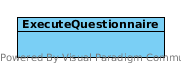
\includegraphics[scale=4, max width=\textwidth, max height=\myheight]{../img/diagrammiClassi/client/view/student/ExecuteQuestionnaire.png}
				\caption{Diagramma classe - client::view::student::ExecuteQuestionnaire}
			\end{figure}
		\end{center}\begin{description}
\item[Descrizione] \hfill \\
 La classe che si occupa della visualizzazione di un questionario in esecuzione
\end{description}

\vspace{0.5cm}
\hypertarget{client::view::student::ExecuteQuestion}{}
\subsubsubsection[ExecuteQuestion]{client::view::student::ExecuteQuestion}
\begin{center}
			\begin{figure}[H]
				\centering 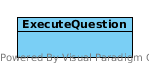
\includegraphics[scale=4, max width=\textwidth, max height=\myheight]{../img/diagrammiClassi/client/view/student/ExecuteQuestion.png}
				\caption{Diagramma classe - client::view::student::ExecuteQuestion}
			\end{figure}
		\end{center}\begin{description}
\item[Descrizione] \hfill \\
 La classe che si occupa della visualizzazione una domanda in esecuzione
\end{description}

\vspace{0.5cm}
\hypertarget{client::view::student::Tags}{}
\subsubsubsection[Tags]{client::view::student::Tags}
\begin{center}
			\begin{figure}[H]
				\centering 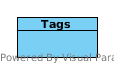
\includegraphics[scale=4, max width=\textwidth, max height=\myheight]{../img/diagrammiClassi/client/view/student/Tags.png}
				\caption{Diagramma classe - client::view::student::Tags}
			\end{figure}
		\end{center}\begin{description}
\item[Descrizione] \hfill \\
 La classe che si occupa della visualizzazione del albero dei argomenti per ricercare un questionario navigando attraverso gli argomenti presenti
\end{description}

\vspace{0.5cm}
\hypertarget{client::view::student::User}{}
\subsubsubsection[User]{client::view::student::User}
\begin{center}
			\begin{figure}[H]
				\centering 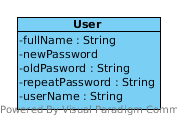
\includegraphics[scale=4, max width=\textwidth, max height=\myheight]{../img/diagrammiClassi/client/view/student/User.png}
				\caption{Diagramma classe - client::view::student::User}
			\end{figure}
		\end{center}\begin{description}
\item[Descrizione] \hfill \\
 La classe che si occupa della visualizzazione della gestione del profilo
\item[Attributi] \hfill \\
 \vspace{-7mm}
\begin{itemize}
\item fullName : String (contiene il nuovo nome  inserito dall'utente )
\item newPassword : String (contiene la nuova password inserita dall'utente )
\item oldPasword : String (contiene la vecchia password inserita dall'utente )
\item repeatPassword : String (contiene la nuova password inserita seconda volta dall'utente )
\item userName : String (contiene il nuovo userName inserito dall'utente )
\end{itemize}

\end{description}

\vspace{0.5cm}
\hypertarget{client::view::student::Home}{}
\subsubsubsection[Home]{client::view::student::Home}
\begin{center}
			\begin{figure}[H]
				\centering 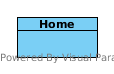
\includegraphics[scale=4, max width=\textwidth, max height=\myheight]{../img/diagrammiClassi/client/view/student/Home.png}
				\caption{Diagramma classe - client::view::student::Home}
			\end{figure}
		\end{center}\begin{description}
\item[Descrizione] \hfill \\
 La classe che si occupa della visualizzazione della home page
\end{description}

\vspace{0.5cm}
\subsubsection{client::view::teacher}
È il package che contiene tutte le classi che costituiscono la view della porzione di client per un docente. Ogni componente si occupa della visualizzazione di una particolare porzione dell'interfaccia di un docente.\begin{center}
		\begin{figure}[H]
			\centering 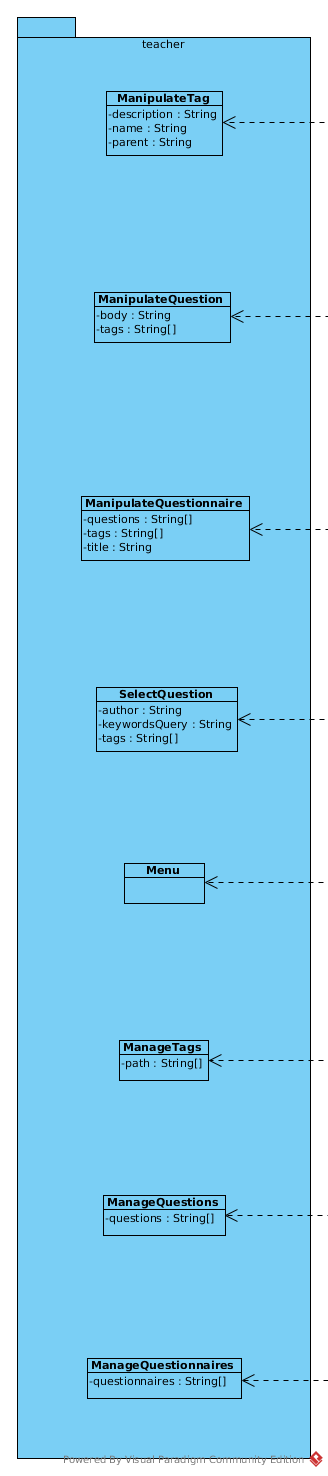
\includegraphics[scale=4, max width=\textwidth, max height=\myheight]{../img/diagrammiClassi/client/view/teacher.png}
			\caption{Diagramma package - client::view::teacher}
		\end{figure}
	\end{center}\hypertarget{client::view::teacher::ManipulateTag}{}
\subsubsubsection[ManipulateTag]{client::view::teacher::ManipulateTag}
\begin{center}
			\begin{figure}[H]
				\centering 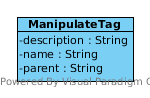
\includegraphics[scale=4, max width=\textwidth, max height=\myheight]{../img/diagrammiClassi/client/view/teacher/ManipulateTag.png}
				\caption{Diagramma classe - client::view::teacher::ManipulateTag}
			\end{figure}
		\end{center}\begin{description}
\item[Descrizione] \hfill \\
 La classe view per la gestione del argomento
\item[Attributi] \hfill \\
 \vspace{-7mm}
\begin{itemize}
\item description : String (contiene la descrizione dell'argomento)
\item name : String (contiene il nome dell'argomento)
\item parent : String (contiene il nome del padre dell'argomento)
\end{itemize}

\end{description}

\vspace{0.5cm}
\hypertarget{client::view::teacher::ManipulateQuestion}{}
\subsubsubsection[ManipulateQuestion]{client::view::teacher::ManipulateQuestion}
\begin{center}
			\begin{figure}[H]
				\centering 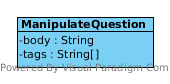
\includegraphics[scale=4, max width=\textwidth, max height=\myheight]{../img/diagrammiClassi/client/view/teacher/ManipulateQuestion.png}
				\caption{Diagramma classe - client::view::teacher::ManipulateQuestion}
			\end{figure}
		\end{center}\begin{description}
\item[Descrizione] \hfill \\
 La classe view che si occupa delle visualizzazione della gestione della domanda
\item[Attributi] \hfill \\
 \vspace{-7mm}
\begin{itemize}
\item body : String (contiene il corpo della domanda)
\item tags : String[] (contiene la lista degli argomenti della domanda)
\end{itemize}

\end{description}

\vspace{0.5cm}
\hypertarget{client::view::teacher::ManipulateQuestionnaire}{}
\subsubsubsection[ManipulateQuestionnaire]{client::view::teacher::ManipulateQuestionnaire}
\begin{center}
			\begin{figure}[H]
				\centering 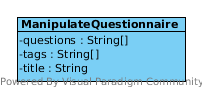
\includegraphics[scale=4, max width=\textwidth, max height=\myheight]{../img/diagrammiClassi/client/view/teacher/ManipulateQuestionnaire.png}
				\caption{Diagramma classe - client::view::teacher::ManipulateQuestionnaire}
			\end{figure}
		\end{center}\begin{description}
\item[Descrizione] \hfill \\
 La classe view che si occupa della visualizzazione della gestione del questionario 
\item[Attributi] \hfill \\
 \vspace{-7mm}
\begin{itemize}
\item questions : String[] (contiene la lista  delle domande del questionario)
\item tags : String[] (contiene la lista degli argomenti del questionario)
\item title : String (contiene il titolo del questionario)
\end{itemize}

\end{description}

\vspace{0.5cm}
\hypertarget{client::view::teacher::SelectQuestion}{}
\subsubsubsection[SelectQuestion]{client::view::teacher::SelectQuestion}
\begin{center}
			\begin{figure}[H]
				\centering 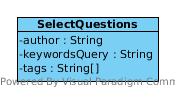
\includegraphics[scale=4, max width=\textwidth, max height=\myheight]{../img/diagrammiClassi/client/view/teacher/SelectQuestion.png}
				\caption{Diagramma classe - client::view::teacher::SelectQuestion}
			\end{figure}
		\end{center}\begin{description}
\item[Descrizione] \hfill \\
 La classe view che si occupa della visualizzazione di selezione delle domande
\item[Attributi] \hfill \\
 \vspace{-7mm}
\begin{itemize}
\item author : String (contiene il nome del autore della domanda)
\item keywordsQuery : String (contiene le parole chiave della ricerca)
\item tags : String[] (contiene la lista degli argomenti della domanda)
\end{itemize}

\end{description}

\vspace{0.5cm}
\hypertarget{client::view::teacher::Menu}{}
\subsubsubsection[Menu]{client::view::teacher::Menu}
\begin{center}
			\begin{figure}[H]
				\centering \includegraphics[scale=4, max width=\textwidth, max height=\myheight]{../img/diagrammiClassi/client/view/teacher/Menu.png}
				\caption{Diagramma classe - client::view::teacher::Menu}
			\end{figure}
		\end{center}\begin{description}
\item[Descrizione] \hfill \\
 La classe view che si occupa della visualizzazione del menu di navigazione per le azioni docente
\end{description}

\vspace{0.5cm}
\hypertarget{client::view::teacher::ManageTags}{}
\subsubsubsection[ManageTags]{client::view::teacher::ManageTags}
\begin{center}
			\begin{figure}[H]
				\centering 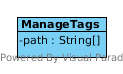
\includegraphics[scale=4, max width=\textwidth, max height=\myheight]{../img/diagrammiClassi/client/view/teacher/ManageTags.png}
				\caption{Diagramma classe - client::view::teacher::ManageTags}
			\end{figure}
		\end{center}\begin{description}
\item[Descrizione] \hfill \\
 La classe view che si occupa della visualizzazione dell'albero degli argomenti per selezionare un eventuale argomento da gestire
\item[Attributi] \hfill \\
 \vspace{-7mm}
\begin{itemize}
\item path : String[] (rapresenta la posizione del tag nella gerarchia completa dei tag sotto forma di percorso a partire dal tag radice)
\end{itemize}

\end{description}

\vspace{0.5cm}
\hypertarget{client::view::teacher::ManageQuestions}{}
\subsubsubsection[ManageQuestions]{client::view::teacher::ManageQuestions}
\begin{center}
			\begin{figure}[H]
				\centering 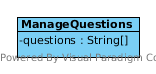
\includegraphics[scale=4, max width=\textwidth, max height=\myheight]{../img/diagrammiClassi/client/view/teacher/ManageQuestions.png}
				\caption{Diagramma classe - client::view::teacher::ManageQuestions}
			\end{figure}
		\end{center}\begin{description}
\item[Descrizione] \hfill \\
 La classe view che si occupa della visualizzazione della lista delle proprie domande per selezionare la domanda da gestire
\item[Attributi] \hfill \\
 \vspace{-7mm}
\begin{itemize}
\item questions : String[] (contiene la lista  delle domande create dal docente)
\end{itemize}

\end{description}

\vspace{0.5cm}
\hypertarget{client::view::teacher::ManageQuestionnaires}{}
\subsubsubsection[ManageQuestionnaires]{client::view::teacher::ManageQuestionnaires}
\begin{center}
			\begin{figure}[H]
				\centering 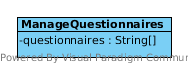
\includegraphics[scale=4, max width=\textwidth, max height=\myheight]{../img/diagrammiClassi/client/view/teacher/ManageQuestionnaires.png}
				\caption{Diagramma classe - client::view::teacher::ManageQuestionnaires}
			\end{figure}
		\end{center}\begin{description}
\item[Descrizione] \hfill \\
 La classe view che si occupa della visualizzazione della lista dei propri questionari per selezionare il questionario da gestire
\item[Attributi] \hfill \\
 \vspace{-7mm}
\begin{itemize}
\item questionnaires : String[] (contiene la lista  dei questionari creati dal docente)
\end{itemize}

\end{description}

\vspace{0.5cm}
\subsubsection{client::view::admin}
È il package che contiene tutte le classi che costituiscono la view della porzione di client per un amministratore. Ogni componente si occupa della visualizzazione di una particolare porzione dell'interfaccia di un amministratore.\begin{center}
		\begin{figure}[H]
			\centering 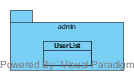
\includegraphics[scale=4, max width=\textwidth, max height=\myheight]{../img/diagrammiClassi/client/view/admin.png}
			\caption{Diagramma package - client::view::admin}
		\end{figure}
	\end{center}\hypertarget{client::view::admin::UsersList}{}
\subsubsubsection[UsersList]{client::view::admin::UsersList}
\begin{center}
			\begin{figure}[H]
				\centering 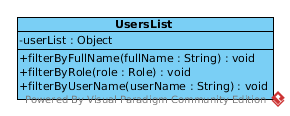
\includegraphics[scale=4, max width=\textwidth, max height=\myheight]{../img/diagrammiClassi/client/view/admin/UsersList.png}
				\caption{Diagramma classe - client::view::admin::UsersList}
			\end{figure}
		\end{center}\begin{description}
\item[Descrizione] \hfill \\
 La classe che si occupa della visualizzazione della lista degli utenti.Consente di applicare un filtro ai risultari tra FullName, Role, UserName per la selezione di un utente per la gestione delle sue informazioni.
\item[Attributi] \hfill \\
 \vspace{-7mm}
\begin{itemize}
\item usersList : Object (contiene la lista degli utenti da stampare)
\end{itemize}

\item[Metodi] \hfill \\
 \vspace{-7mm}
\begin{itemize}
\item filterByFullName(fullName : String) : void (Filtra la lista dei utenti per nome in base al parametro fullName passato)\begin{itemize}
\item fullName (Contiene il nome su cui eseguire il filtro)
\end{itemize}

\item filterByRole(role : Role) : void (Filtra la lista dei utenti per ruolo in base al parametro role passato)\begin{itemize}
\item role (Contiene il ruolo su cui fare filtro)
\end{itemize}

\item filterByUserName(userName : String) : void (Filtra la lista dei utenti per userName in base al parametro userName passato)\begin{itemize}
\item userName (Contiene il username su cui eseguire il filtro)
\end{itemize}

\end{itemize}

\end{description}

\vspace{0.5cm}
\hypertarget{client::view::admin::Menu}{}
\subsubsubsection[Menu]{client::view::admin::Menu}
\begin{center}
			\begin{figure}[H]
				\centering \includegraphics[scale=4, max width=\textwidth, max height=\myheight]{../img/diagrammiClassi/client/view/admin/Menu.png}
				\caption{Diagramma classe - client::view::admin::Menu}
			\end{figure}
		\end{center}\begin{description}
\item[Descrizione] \hfill \\
 La classe che si occupa della visualizzazione del menu di navigazione dell'amministratore
\end{description}

\vspace{0.5cm}
\subsection{client::model}
E' il package che contiene le classi dei modelli di dati utilizzati
dal client e i servizi che mettono in comunicazione esso con il server
attraverso i diversi servizi REST.\begin{center}
		\begin{figure}[H]
			\centering 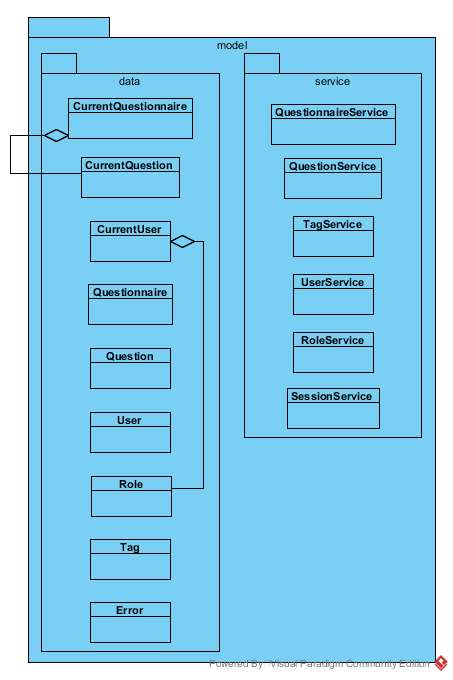
\includegraphics[scale=4, max width=\textwidth, max height=\myheight]{../img/diagrammiClassi/client/model.png}
			\caption{Diagramma package - client::model}
		\end{figure}
	\end{center}\subsubsection{client::model::data}
Questo package si occupa della modellazione dei dati utili al client.\begin{center}
		\begin{figure}[H]
			\centering 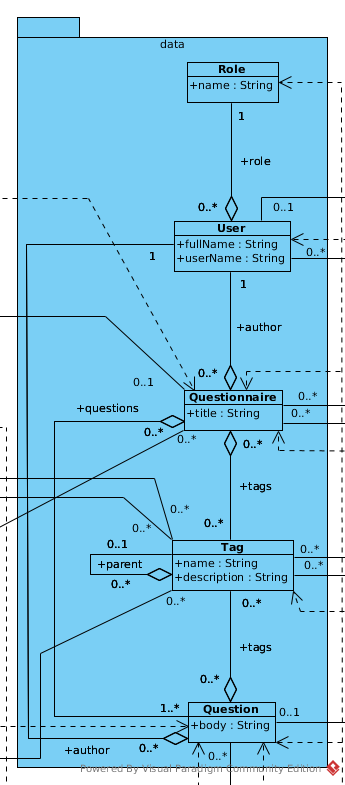
\includegraphics[scale=4, max width=\textwidth, max height=\myheight]{../img/diagrammiClassi/client/model/data.png}
			\caption{Diagramma package - client::model::data}
		\end{figure}
	\end{center}\hypertarget{client::model::data::Questionnaire}{}
\subsubsubsection[Questionnaire]{client::model::data::Questionnaire}
\begin{center}
			\begin{figure}[H]
				\centering 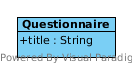
\includegraphics[scale=4, max width=\textwidth, max height=\myheight]{../img/diagrammiClassi/client/model/data/Questionnaire.png}
				\caption{Diagramma classe - client::model::data::Questionnaire}
			\end{figure}
		\end{center}\begin{description}
\item[Descrizione] \hfill \\
 Questa classe modella il tipo di dato "questionario" nella rappresentazione locale dei dati lato client
\item[Relazioni con altre classi] \hfill \\
 \vspace{-7mm}
\begin{description}
\item[\hyperlink{client::model::data::Tag}{client::model::data::Tag}] \hfill \\
 Relazione uscente, raccolta degli argomenti del questionario
\item[\hyperlink{client::model::data::User}{client::model::data::User}] \hfill \\
 Relazione uscente, riferimento all'autore del questionario
\item[\hyperlink{client::model::data::Question}{client::model::data::Question}] \hfill \\
 Relazione uscente, insieme di riferimenti a Question
\item[\hyperlink{client::controller::teacher::ManipulateQuestionnaire}{client::controller::teacher::ManipulateQuestionnaire}] \hfill \\
 Relazione entrante, oggetto che rappresenta un questionario
\item[\hyperlink{client::controller::teacher::ManageQuestionnaires}{client::controller::teacher::ManageQuestionnaires}] \hfill \\
 Relazione entrante, lista di questionari
\item[\hyperlink{client::controller::student::Questionnaires}{client::controller::student::Questionnaires}] \hfill \\
 Relazione entrante, lista di questionari
\item[\hyperlink{client::controller::student::Tags}{client::controller::student::Tags}] \hfill \\
 Relazione entrante, lista di questionari
\end{description}

\item[Attributi] \hfill \\
 \vspace{-7mm}
\begin{itemize}
\item questions : Question[] (Insieme di riferimenti a Question)
\item tags : Tag[] (Raccolta degli argomenti del questionario)
\item author : User (Riferimento all'autore del questionario)
\item title : String (Nome del questionario)
\end{itemize}

\end{description}

\vspace{0.5cm}
\hypertarget{client::model::data::Question}{}
\subsubsubsection[Question]{client::model::data::Question}
\begin{center}
			\begin{figure}[H]
				\centering 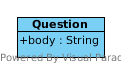
\includegraphics[scale=4, max width=\textwidth, max height=\myheight]{../img/diagrammiClassi/client/model/data/Question.png}
				\caption{Diagramma classe - client::model::data::Question}
			\end{figure}
		\end{center}\begin{description}
\item[Descrizione] \hfill \\
 Questa classe modella il tipo di dato "domanda" nella rappresentazione locale dei dati lato client
\item[Relazioni con altre classi] \hfill \\
 \vspace{-7mm}
\begin{description}
\item[\hyperlink{client::model::data::Questionnaire}{client::model::data::Questionnaire}] \hfill \\
 Relazione entrante, insieme di riferimenti a Question
\item[\hyperlink{client::model::data::Tag}{client::model::data::Tag}] \hfill \\
 Relazione uscente, lista di argomenti  
\item[\hyperlink{client::model::data::User}{client::model::data::User}] \hfill \\
 Relazione uscente, chi ha creato la domanda
\item[\hyperlink{client::controller::teacher::ManipulateQuestion}{client::controller::teacher::ManipulateQuestion}] \hfill \\
 Relazione entrante, oggetto che rappresenta una singola domanda
\item[\hyperlink{client::controller::teacher::ManageQuestions}{client::controller::teacher::ManageQuestions}] \hfill \\
 Relazione entrante, lista delle domande create da uno stesso docente
\end{description}

\item[Attributi] \hfill \\
 \vspace{-7mm}
\begin{itemize}
\item body : String (E' la rappresentazione testuale della domanda)
\item author : User  (Chi ha creato la domanda)
\item tags  : Tag[] (Lista di argomenti  )
\end{itemize}

\end{description}

\vspace{0.5cm}
\hypertarget{client::model::data::Tag}{}
\subsubsubsection[Tag]{client::model::data::Tag}
\begin{center}
			\begin{figure}[H]
				\centering 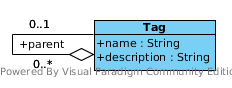
\includegraphics[scale=4, max width=\textwidth, max height=\myheight]{../img/diagrammiClassi/client/model/data/Tag.png}
				\caption{Diagramma classe - client::model::data::Tag}
			\end{figure}
		\end{center}\begin{description}
\item[Descrizione] \hfill \\
 Questa classe modella il tag argomento di un questionario e/o di una domanda nella rappresentazione locale dei dati lato client
\item[Relazioni con altre classi] \hfill \\
 \vspace{-7mm}
\begin{description}
\item[\hyperlink{client::model::data::Questionnaire}{client::model::data::Questionnaire}] \hfill \\
 Relazione entrante, raccolta degli argomenti del questionario
\item[\hyperlink{client::model::data::Question}{client::model::data::Question}] \hfill \\
 Relazione entrante, lista di argomenti  
\item[\hyperlink{client::controller::teacher::ManipulateTag}{client::controller::teacher::ManipulateTag}] \hfill \\
 Relazione entrante, rappresenta il nome e la descrizione di un argomento
\item[\hyperlink{client::controller::teacher::SelectQuestion}{client::controller::teacher::SelectQuestion}] \hfill \\
 Relazione entrante, lista degli argomenti associati ad un questionario
\item[\hyperlink{client::controller::teacher::ManageTags}{client::controller::teacher::ManageTags}] \hfill \\
 Relazione entrante, lista di argomenti visti come un cammino che parte dalla radice fino al figlio selezionato
\item[\hyperlink{client::controller::student::Questionnaires}{client::controller::student::Questionnaires}] \hfill \\
 Relazione entrante, lista degli argomenti trattati in un questionario
\item[\hyperlink{client::controller::student::Tags}{client::controller::student::Tags}] \hfill \\
 Relazione entrante, lista di argomenti visti come un cammino che parte dalla radice fino al figlio selezionato
\end{description}

\item[Attributi] \hfill \\
 \vspace{-7mm}
\begin{itemize}
\item parent : Tag (Argomento padre )
\item name : String (Nome dell'argomento)
\item description : String (Descrizione dell'argomento)
\end{itemize}

\end{description}

\vspace{0.5cm}
\hypertarget{client::model::data::Role}{}
\subsubsubsection[Role]{client::model::data::Role}
\begin{center}
			\begin{figure}[H]
				\centering 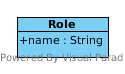
\includegraphics[scale=4, max width=\textwidth, max height=\myheight]{../img/diagrammiClassi/client/model/data/Role.png}
				\caption{Diagramma classe - client::model::data::Role}
			\end{figure}
		\end{center}\begin{description}
\item[Descrizione] \hfill \\
 Questa classe modella il ruolo e i permessi di un utente autenticato nel sistema
\item[Relazioni con altre classi] \hfill \\
 \vspace{-7mm}
\begin{description}
\item[\hyperlink{client::model::data::User}{client::model::data::User}] \hfill \\
 Relazione entrante, ruolo dell'utente
\end{description}

\item[Attributi] \hfill \\
 \vspace{-7mm}
\begin{itemize}
\item name : String (E' il ruolo che un utente può assumere)
\end{itemize}

\end{description}

\vspace{0.5cm}
\hypertarget{client::model::data::User}{}
\subsubsubsection[User]{client::model::data::User}
\begin{center}
			\begin{figure}[H]
				\centering 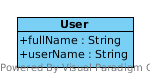
\includegraphics[scale=4, max width=\textwidth, max height=\myheight]{../img/diagrammiClassi/client/model/data/User.png}
				\caption{Diagramma classe - client::model::data::User}
			\end{figure}
		\end{center}\begin{description}
\item[Descrizione] \hfill \\
 Questa classe modella le informazioni del profilo di un utente autenticato nel sistema
\item[Relazioni con altre classi] \hfill \\
 \vspace{-7mm}
\begin{description}
\item[\hyperlink{client::model::data::Questionnaire}{client::model::data::Questionnaire}] \hfill \\
 Relazione entrante, riferimento all'autore del questionario
\item[\hyperlink{client::model::data::Role}{client::model::data::Role}] \hfill \\
 Relazione uscente, ruolo dell'utente
\item[\hyperlink{client::model::data::Question}{client::model::data::Question}] \hfill \\
 Relazione entrante, chi ha creato la domanda
\item[\hyperlink{client::controller::admin::UsersList}{client::controller::admin::UsersList}] \hfill \\
 Relazione entrante, lista di utenti
\item[\hyperlink{client::controller::student::User}{client::controller::student::User}] \hfill \\
 Relazione entrante, utente loggato
\end{description}

\item[Attributi] \hfill \\
 \vspace{-7mm}
\begin{itemize}
\item role : Role (ruolo dell'utente)
\item fullName : String (nome completo dell'utente)
\item userName : String (userName dell'utente)
\end{itemize}

\end{description}

\vspace{0.5cm}
\subsubsection{client::model::service}
Questo package contiene le classi che gestiscono il recupero dei dati, che siano essi salvati in locale o recuperabili dall'interfaccia server tramite le Api REST.\begin{center}
		\begin{figure}[H]
			\centering 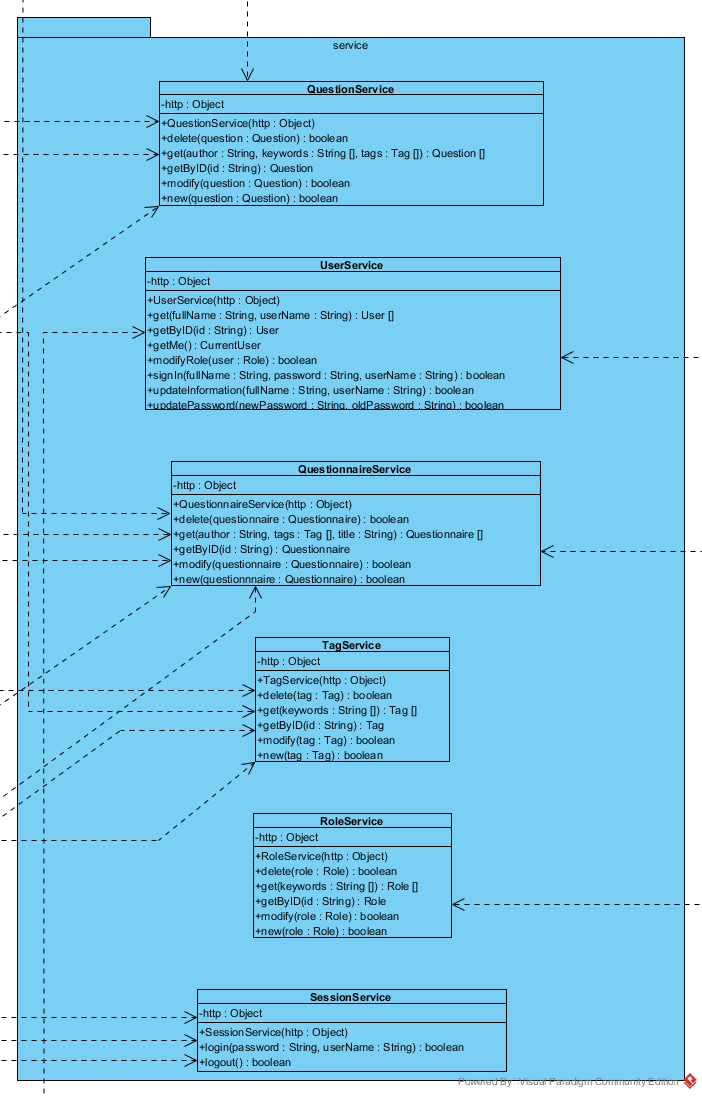
\includegraphics[scale=4, max width=\textwidth, max height=\myheight]{../img/diagrammiClassi/client/model/service.png}
			\caption{Diagramma package - client::model::service}
		\end{figure}
	\end{center}\hypertarget{client::model::service::SessionService}{}
\subsubsubsection[SessionService]{client::model::service::SessionService}
\begin{center}
			\begin{figure}[H]
				\centering 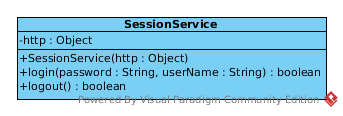
\includegraphics[scale=4, max width=\textwidth, max height=\myheight]{../img/diagrammiClassi/client/model/service/SessionService.png}
				\caption{Diagramma classe - client::model::service::SessionService}
			\end{figure}
		\end{center}\begin{description}
\item[Descrizione] \hfill \\
 Questa classe fornisce al client i servizi relativi  alle credenziali accesso di un utente
\item[Attributi] \hfill \\
 \vspace{-7mm}
\begin{itemize}
\item http : Object (Oggetto del servizio offerto da angulajs per le richieste http)
\end{itemize}

\item[Metodi] \hfill \\
 \vspace{-7mm}
\begin{itemize}
\item SessionService(http : Object) (Costruttore della classe)\begin{itemize}
\item http (Oggetto del servizio offerto da angulajs per le richieste http)
\end{itemize}

\item login(password : String, userName : String) : boolean (Controlla se i parametri dell'utente sono presenti)\begin{itemize}
\item password (Contiene la password inserita dall'utente)
\item userName (Contiene l'username inserito dall'utente)
\end{itemize}

\item logout() : boolean (Chiude la sessione dell'utente)
\end{itemize}

\end{description}

\vspace{0.5cm}
\hypertarget{client::model::service::UserService}{}
\subsubsubsection[UserService]{client::model::service::UserService}
\begin{center}
			\begin{figure}[H]
				\centering 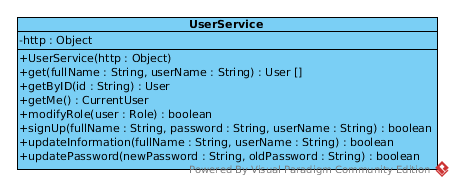
\includegraphics[scale=4, max width=\textwidth, max height=\myheight]{../img/diagrammiClassi/client/model/service/UserService.png}
				\caption{Diagramma classe - client::model::service::UserService}
			\end{figure}
		\end{center}\begin{description}
\item[Descrizione] \hfill \\
 Questa classe fornisce al client i servizi relativi al profilo 
\item[Attributi] \hfill \\
 \vspace{-7mm}
\begin{itemize}
\item http : Object (Oggetto del servizio offerto da angulajs per le richieste http)
\end{itemize}

\item[Metodi] \hfill \\
 \vspace{-7mm}
\begin{itemize}
\item UserService(http : Object) (Il costruttore del servizio)\begin{itemize}
\item http (Oggetto del servizio offerto da angulajs per le richieste http)
\end{itemize}

\item get(fullName : String, userName : String) : User[] (Metodo che ritorna la lista dei utenti in base ai parametri passati)\begin{itemize}
\item fullName (Contiene il nome del utente da ricercare )
\item userName (Contiene il username dell'utente da ricercare )
\end{itemize}

\item getByID(id : String) : User (Metodo che ritorna dal server un utente per id)\begin{itemize}
\item id (Contiene id dell'utente da ricercare )
\end{itemize}

\item getMe() : CurrentUser (Metodo che ritorna dal server i dati del utente corrente)
\item signIn(fullName : String, password : String, userName : String) : boolean (Metodo per registrazione del utente nel nostro sistema)\begin{itemize}
\item fullName (Contiene il nome del nuovo utente)
\item password (Contiene la password del nuovo utente)
\item userName (Contiene il username del nuovo utente)
\end{itemize}

\item updateInformation(fullName : String, userName : String) : boolean (Metodo per cambiare proprie informazioni di profilo sul server)\begin{itemize}
\item fullName (Contiene il nuovo nome dell'utente)
\item userName (Contiene il nuovo username dell'utente)
\end{itemize}

\item updatePassword(newPassword : String, oldPassword : String) : boolean (Metodo per cambio password nel sistema)\begin{itemize}
\item newPassword (Contiene il nuovo password dell'utente)
\item oldPassword (Contiene la vecchia password dell'utente)
\end{itemize}

\item modifyRole(user : User, role : Role) : boolean (Metodo per cambio del ruolo dell'utente sul server)\begin{itemize}
\item user (Contiene l'utente il cui ruolo deve essere cambiato)
\item role (Contiene il nuovo ruolo dell'utente)
\end{itemize}

\end{itemize}

\end{description}

\vspace{0.5cm}
\hypertarget{client::model::service::TagService}{}
\subsubsubsection[TagService]{client::model::service::TagService}
\begin{center}
			\begin{figure}[H]
				\centering 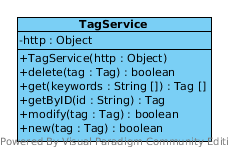
\includegraphics[scale=4, max width=\textwidth, max height=\myheight]{../img/diagrammiClassi/client/model/service/TagService.png}
				\caption{Diagramma classe - client::model::service::TagService}
			\end{figure}
		\end{center}\begin{description}
\item[Descrizione] \hfill \\
 Questa classe fornisce al client i servizi relativi alla modifica, cancellazione e lettura e inserimento dei tag presenti nel sistema
\item[Attributi] \hfill \\
 \vspace{-7mm}
\begin{itemize}
\item http : Object (Oggetto del servizio offerto da angulajs per le richieste http)
\end{itemize}

\item[Metodi] \hfill \\
 \vspace{-7mm}
\begin{itemize}
\item TagService(http : Object) (Il costruttore del servizio)\begin{itemize}
\item http (Oggetto del servizio offerto da angulajs per le richieste http)
\end{itemize}

\item delete(tag : Tag) : boolean (Metodo che riceve un oggetto di tipo Tag e tramite API REST del server cancella tale oggetto dal server)\begin{itemize}
\item tag (Contiene l'argomento da eliminare)
\end{itemize}

\item get(keywords : String[]) : Tag [] (Metodo che ritorna una lista dei Tag in base alle parole chiave ricevute dal parametro keywords)\begin{itemize}
\item keywords (Contiene la lista di parole chiave per ricercare gli argomenti)
\end{itemize}

\item getByID(id : String) : Tag (Metodo che ritorna Tag (argomento) per id)\begin{itemize}
\item id (Contiene id dell'argomento da ricercare)
\end{itemize}

\item modify(tag : Tag) : boolean (Metodo che riceve un oggetto di tipo Tag e tramite API REST del server modifica tale oggetto sul server)\begin{itemize}
\item tag (Contiene l'argomento da modificare)
\end{itemize}

\item new(tag : Tag) : boolean (Metodo che riceve un oggetto di tipo Tag e tramite API REST del server crea un nuovo oggetto Tag sul server)\begin{itemize}
\item tag (Contiene il nuovo argomento da creare)
\end{itemize}

\end{itemize}

\end{description}

\vspace{0.5cm}
\hypertarget{client::model::service::RoleService}{}
\subsubsubsection[RoleService]{client::model::service::RoleService}
\begin{center}
			\begin{figure}[H]
				\centering 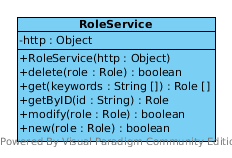
\includegraphics[scale=4, max width=\textwidth, max height=\myheight]{../img/diagrammiClassi/client/model/service/RoleService.png}
				\caption{Diagramma classe - client::model::service::RoleService}
			\end{figure}
		\end{center}\begin{description}
\item[Descrizione] \hfill \\
 Questa classe fornisce al client i servizi necessari per la gestione dei ruoli
\item[Attributi] \hfill \\
 \vspace{-7mm}
\begin{itemize}
\item http : Object (Oggetto del servizio offerto da angulajs per le richieste http)
\end{itemize}

\item[Metodi] \hfill \\
 \vspace{-7mm}
\begin{itemize}
\item RoleService(http : Object) (Il costruttore del servizio)\begin{itemize}
\item http (Oggetto del servizio offerto da angulajs per le richieste http)
\end{itemize}

\item delete(role : Role) : boolean (Metodo che riceve un oggetto di tipo Role e tramite API REST del server cancella tale oggetto dal server)\begin{itemize}
\item role (Contiene il ruolo da eliminare)
\end{itemize}

\item get(keywords : String[]) : Role [] (Metodo che ritorna la lista dei ruoli in base alle parole chive passate tramite parametro keywords)\begin{itemize}
\item keywords (Contiene la lista di parole chiave per ricercare il ruolo)
\end{itemize}

\item getByID(id : String) : Role (Metodo che ritorna un ruolo per id)\begin{itemize}
\item id (Contiene id del ruolo da ricercare)
\end{itemize}

\item modify(role : Role) : boolean (Metodo che riceve un oggetto di tipo role e tramite API REST del server cambia tale oggetto sul server)\begin{itemize}
\item role (Contiene il ruolo da modificare)
\end{itemize}

\item new(role : Role) : boolean (Metodo che riceve un oggetto di tipo Role e tramite API REST del server crea un nuovo oggetto sul server)\begin{itemize}
\item role (Contiene il nuovo ruolo da creare)
\end{itemize}

\end{itemize}

\end{description}

\vspace{0.5cm}
\hypertarget{client::model::service::QuestionService}{}
\subsubsubsection[QuestionService]{client::model::service::QuestionService}
\begin{center}
			\begin{figure}[H]
				\centering 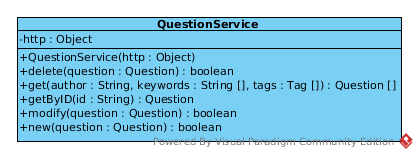
\includegraphics[scale=4, max width=\textwidth, max height=\myheight]{../img/diagrammiClassi/client/model/service/QuestionService.png}
				\caption{Diagramma classe - client::model::service::QuestionService}
			\end{figure}
		\end{center}\begin{description}
\item[Descrizione] \hfill \\
 Questa classe fornisce al client i servizi necessari alla gestione delle domande
\item[Attributi] \hfill \\
 \vspace{-7mm}
\begin{itemize}
\item http : Object (Oggetto del servizio offerto da angulajs per le richieste http)
\end{itemize}

\item[Metodi] \hfill \\
 \vspace{-7mm}
\begin{itemize}
\item QuestionService(http : Object) (Il costruttore del servizio)\begin{itemize}
\item http (Oggetto del servizio offerto da angulajs per le richieste http)
\end{itemize}

\item delete(question : Question) : boolean (Metodo che prende come parametro un oggetto di tipo Question e tramite API REST del server cancella tale oggetto dal server)\begin{itemize}
\item question (Contiene la domanda da eliminare)
\end{itemize}

\item get(author : String, keywords : String[], tags : Tag[]) : Question[] (Metodo che ritorna una lista delle domande dal server in base ai parametri passati al metodo)\begin{itemize}
\item author (Contiene il nome dell'autore della domanda da ricercare )
\item keywords (Contiene la lista di parole chiave per ricercare una domanda)
\item tags (Contiene la lista degli argomenti per ricercare una domanda)
\end{itemize}

\item getByID(id : String) : Question[] (Metodo che ritorna una domanda dal server per id)\begin{itemize}
\item id (ID della Question)
\end{itemize}

\item modify(question : Question) : boolean (Metodo che prende come parametro un oggetto di tipo question e tramite API REST del server modifica tale domanda sul server)\begin{itemize}
\item question (Contiene la domanda da modificare)
\end{itemize}

\item new(question : Question) : boolean (Metodo che prende come parametro un oggetto di tipo question e tramite API REST del server crea una nuova domanda sul server)\begin{itemize}
\item question (Contiene la nuova domanda da creare)
\end{itemize}

\end{itemize}

\end{description}

\vspace{0.5cm}
\hypertarget{client::model::service::QuestionnaireService}{}
\subsubsubsection[QuestionnaireService]{client::model::service::QuestionnaireService}
\begin{center}
			\begin{figure}[H]
				\centering 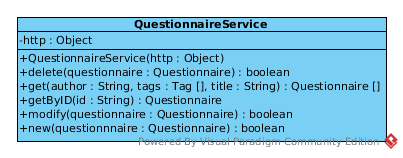
\includegraphics[scale=4, max width=\textwidth, max height=\myheight]{../img/diagrammiClassi/client/model/service/QuestionnaireService.png}
				\caption{Diagramma classe - client::model::service::QuestionnaireService}
			\end{figure}
		\end{center}\begin{description}
\item[Descrizione] \hfill \\
 Questa classe fornisce al client i servizi necessari alla gestione dei questionari
\item[Attributi] \hfill \\
 \vspace{-7mm}
\begin{itemize}
\item http : Object (Oggetto del servizio offerto da angulajs per le richieste http)
\end{itemize}

\item[Metodi] \hfill \\
 \vspace{-7mm}
\begin{itemize}
\item QestionnaireService(http : Object) (Costruttore della classe)\begin{itemize}
\item http (Oggetto del servizio offerto da angulajs per le richieste http)
\end{itemize}

\item delete(questionnaire : Questionnaire) : boolean (Elimina il questionario passato per parametro)\begin{itemize}
\item questionnaire (Contiene il questionario da eliminare)
\end{itemize}

\item get (author : String, tags  : Tag[], title : String) : Questionnaire[] (Ritorna tutti i questionari che sono stati ricercati per autore, argomento e titolo)\begin{itemize}
\item author (Contiene il nome dell'autore del questionario da ricercare)
\item tags  (Contiene la lista degli argomenti per ricercare un questionario)
\item title (Contiene il titolo del questionario da ricercare)
\end{itemize}

\item getByID(id : String) : Questionnaire (Ritorna un questionario ricercato per ID)\begin{itemize}
\item id (contiene id del questionario da ricercare)
\end{itemize}

\item modify(questionnaire : Questionnaire) : boolean (Modifica il questionario passato per argomento)\begin{itemize}
\item questionnaire (Contiene il questionario da modificare)
\end{itemize}

\item new(questionnaire : Questionnaire) : boolean (Crea un nuovo questionario)\begin{itemize}
\item questionnaire (Contiene il nuovo questionario da creare)
\end{itemize}

\end{itemize}

\end{description}

\vspace{0.5cm}
\subsubsection{client::model::util}
Il package che contiene le classi di utilità del client.\begin{center}
		\begin{figure}[H]
			\centering 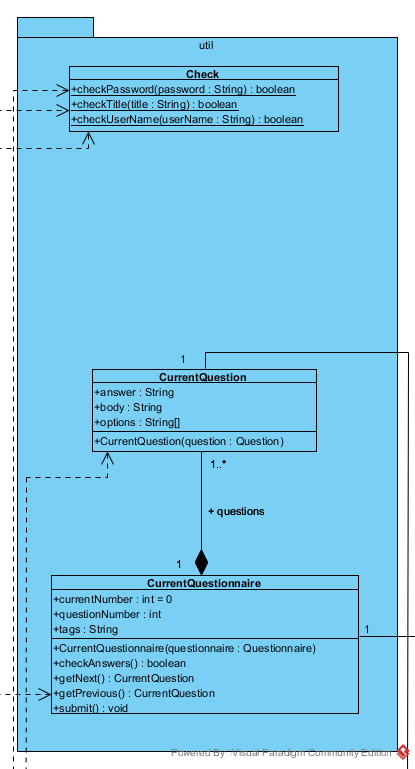
\includegraphics[scale=4, max width=\textwidth, max height=\myheight]{../img/diagrammiClassi/client/model/util.png}
			\caption{Diagramma package - client::model::util}
		\end{figure}
	\end{center}\hypertarget{client::model::util::Check}{}
\subsubsubsection[Check]{client::model::util::Check}
\begin{center}
			\begin{figure}[H]
				\centering 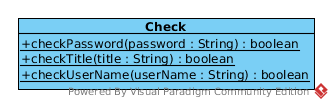
\includegraphics[scale=4, max width=\textwidth, max height=\myheight]{../img/diagrammiClassi/client/model/util/Check.png}
				\caption{Diagramma classe - client::model::util::Check}
			\end{figure}
		\end{center}\begin{description}
\item[Descrizione] \hfill \\
 La classe che controlla se la password,  l'userName o titolo rispettino il formato scelto
\item[Metodi] \hfill \\
 \vspace{-7mm}
\begin{itemize}
\item checkPassword(password : String) : boolean (Metodo che controlla la conformità del parametro passato password al formato scelto per le password)\begin{itemize}
\item password (Contiene la password da controlare  )
\end{itemize}

\item checkUserName(userName : String) : boolean (Metodo che controlla la conformità del parametro passato userName al formato scelto nel sistema per i username)\begin{itemize}
\item userName (Contiene il username da controllare )
\end{itemize}

\item checkTitle(title : String) : boolean (Metodo che controlla la conformità del parametro passato title al formato scelto dal sistema per i titolo)\begin{itemize}
\item title (Contiene il titolo da controllare )
\end{itemize}

\end{itemize}

\end{description}

\vspace{0.5cm}
\hypertarget{client::model::util::CurrentQuestion}{}
\subsubsubsection[CurrentQuestion]{client::model::util::CurrentQuestion}
\begin{center}
			\begin{figure}[H]
				\centering 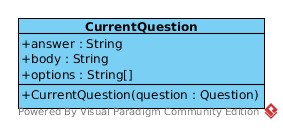
\includegraphics[scale=4, max width=\textwidth, max height=\myheight]{../img/diagrammiClassi/client/model/util/CurrentQuestion.png}
				\caption{Diagramma classe - client::model::util::CurrentQuestion}
			\end{figure}
		\end{center}\begin{description}
\item[Descrizione] \hfill \\
 La classe che modella la domanda in esecuzione
\item[Relazioni con altre classi] \hfill \\
 \vspace{-7mm}
\begin{description}
\item[\hyperlink{client::model::util::CurrentQuestionnaire}{client::model::util::CurrentQuestionnaire}] \hfill \\
 Relazione entrante, domande del questionario corrente
\item[\hyperlink{client::controller::student::ExecuteQuestion}{client::controller::student::ExecuteQuestion}] \hfill \\
 Relazione entrante, domanda corrente
\end{description}

\item[Attributi] \hfill \\
 \vspace{-7mm}
\begin{itemize}
\item body : String (Contiene il corpo della domanda corrente )
\item options : String[] (Contiene la lista delle risposte per la domanda corrente)
\item answer : String (Contiene la risposta alla domanda corrente)
\end{itemize}

\item[Metodi] \hfill \\
 \vspace{-7mm}
\begin{itemize}
\item CurrentQuestion(question : Question) (Il costruttore del CurrentQuestion, ha bisogno per essere costruito del parametro di tipo Question)\begin{itemize}
\item question (Contiene il riferimento all'oggetto Question associato)
\end{itemize}

\end{itemize}

\end{description}

\vspace{0.5cm}
\hypertarget{client::model::util::CurrentQuestionnaire}{}
\subsubsubsection[CurrentQuestionnaire]{client::model::util::CurrentQuestionnaire}
\begin{center}
			\begin{figure}[H]
				\centering 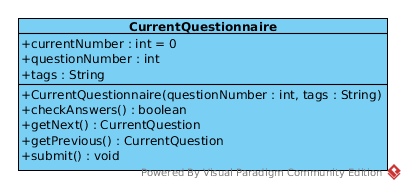
\includegraphics[scale=4, max width=\textwidth, max height=\myheight]{../img/diagrammiClassi/client/model/util/CurrentQuestionnaire.png}
				\caption{Diagramma classe - client::model::util::CurrentQuestionnaire}
			\end{figure}
		\end{center}\begin{description}
\item[Descrizione] \hfill \\
 La classe che modella il questionario in esecuzione
\item[Relazioni con altre classi] \hfill \\
 \vspace{-7mm}
\begin{description}
\item[\hyperlink{client::model::util::CurrentQuestion}{client::model::util::CurrentQuestion}] \hfill \\
 Relazione uscente, domande del questionario corrente
\item[\hyperlink{client::controller::student::ExecuteQuestionnaire}{client::controller::student::ExecuteQuestionnaire}] \hfill \\
 Relazione entrante, istanza del questionario di esecuzione
\end{description}

\item[Attributi] \hfill \\
 \vspace{-7mm}
\begin{itemize}
\item tags : String (Contiene la lista degli argomenti del questionario)
\item currentNumber : int ( Contiene numero della domanda corrente che si sta eseguendo)
\item questionNumber : int (Contiene il numero totale delle domande nel questionario corrente)
\item questions : CurrentQuestion (Domande del questionario corrente)
\end{itemize}

\item[Metodi] \hfill \\
 \vspace{-7mm}
\begin{itemize}
\item getNext () : CurrentQuestion (Metodo che ritorna la prossima domanda)
\item getPrevious() : CurrentQuestion (Metodo che ritorna la domanda precedente)
\item checkAnswers() : boolean (Metodo che controlla che tutte le domande hanno una risposta data)
\item submit() : void (Metodo che controlla con checkAnswers() che ci siano tutte le risposte e poi manda il questionario eseguito al server per il controllo)
\item CurrentQuestionnaire(questionnaire : Questionnaire) (Costruttore della classe CurrentQuestionnaire)\begin{itemize}
\item questionnaire (Il questionario associato al CurrentQuestionnaire)
\end{itemize}

\end{itemize}

\end{description}

\vspace{0.5cm}
\subsection{client::controller}
È il package che contiene le componenti che contengono i
controller dell’applicazione e che incapsulano le funzionalità di two-way data binding tra le View e il Model. In esse è contenuta la logica applicativa riguardante le diverse pagine HTML.\begin{center}
		\begin{figure}[H]
			\centering 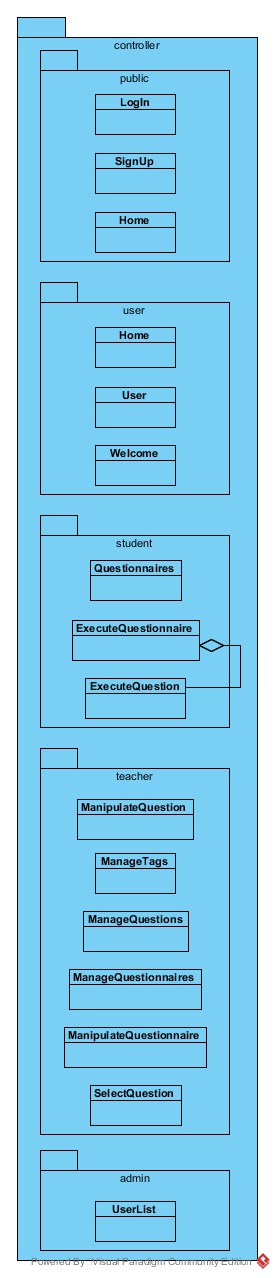
\includegraphics[scale=4, max width=\textwidth, max height=\myheight]{../img/diagrammiClassi/client/controller.png}
			\caption{Diagramma package - client::controller}
		\end{figure}
	\end{center}\subsubsection{client::controller::public}
È il package che contiene tutte le classi che costituiscono i controller della porzione pubblica di un client. Ogni componente si occupa della gestione di una particolare porzione dell'interfaccia di un utente non autenticato che verrà successivamente visualizzata nella corrispondente view.\begin{center}
		\begin{figure}[H]
			\centering 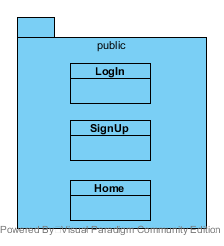
\includegraphics[scale=4, max width=\textwidth, max height=\myheight]{../img/diagrammiClassi/client/controller/public.png}
			\caption{Diagramma package - client::controller::public}
		\end{figure}
	\end{center}\hypertarget{client::controller::public::LogIn}{}
\subsubsubsection[LogIn]{client::controller::public::LogIn}
\begin{center}
			\begin{figure}[H]
				\centering 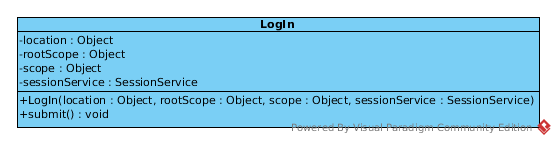
\includegraphics[scale=4, max width=\textwidth, max height=\myheight]{../img/diagrammiClassi/client/controller/public/LogIn.png}
				\caption{Diagramma classe - client::controller::public::LogIn}
			\end{figure}
		\end{center}\begin{description}
\item[Descrizione] \hfill \\
 Classe che gestisce le operazioni e la logica applicativa riguardante la pagina di autenticazione sul client
\item[Utilizzo] \hfill \\
 Viene utilizzata per generare la pagina di autenticazione all’applicazione. Prima della creazione della view viene effettuato un controllo sull’esistenza di una sessione utente. In caso positivo il controller si occuperà di visualizzare la home dell'utente loggato, altrimenti si procederà alla pagina di Login predefinita.
\item[Attributi] \hfill \\
 \vspace{-7mm}
\begin{itemize}
\item location : Object (analizza l'URL nella barra degli indirizzi del browser e lo rende disponibile all'applicazione)
\item rootScope : Object (oggetto identificato dall’elemento con attributo ng-app)
\item scope : Object (oggetto che fa riferimento ad una porzione di model di pertinenza di questo specifico controller)
\item sessionService : SessionService (controlla se un utente ha già una sessione attiva)
\end{itemize}

\item[Metodi] \hfill \\
 \vspace{-7mm}
\begin{itemize}
\item LogIn(rootScope : Object, scope : Object, sessionService : client.service.SessionService) (costruttore della classe)\begin{itemize}
\item rootScope (oggetto identificato dall’elemento con attributo ng-app)
\item scope (oggetto che fa riferimento ad una porzione di model di pertinenza di questo specifico controller)
\item sessionService (Contiene il riferimento verso il servizio della sessione)
\end{itemize}

\item submit() : void (invia lo username e la password dell'utente al server per fare l'autenticazione)
\end{itemize}

\end{description}

\vspace{0.5cm}
\hypertarget{client::controller::public::SignUp}{}
\subsubsubsection[SignUp]{client::controller::public::SignUp}
\begin{center}
			\begin{figure}[H]
				\centering 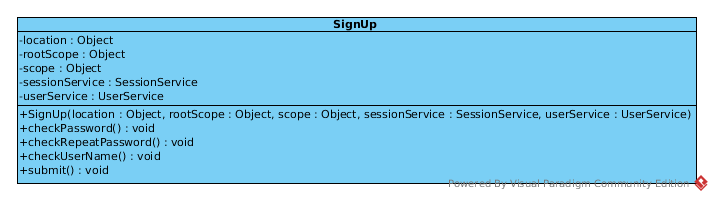
\includegraphics[scale=4, max width=\textwidth, max height=\myheight]{../img/diagrammiClassi/client/controller/public/SignUp.png}
				\caption{Diagramma classe - client::controller::public::SignUp}
			\end{figure}
		\end{center}\begin{description}
\item[Descrizione] \hfill \\
 Classe che gestisce le operazioni e la logica applicativa riguardante la pagina di Registrazione sul client
\item[Utilizzo] \hfill \\
 Deve visualizzare campi per l’inserimento della mail, password, nome e cognome. Deve poter gestire l'eventuale caso di errore se la mail dello studente è già presente nel sistema. Inoltre deve poter gestire il caso in cui di la password dello studente non rispetta i parametri prestabiliti 
\item[Attributi] \hfill \\
 \vspace{-7mm}
\begin{itemize}
\item location : Object (analizza l'URL nella barra degli indirizzi del browser e lo rende disponibile all'applicazione)
\item rootScope : Object (oggetto identificato dall’elemento con attributo ng-app)
\item scope : Object (oggetto che fa riferimento ad una porzione di model di pertinenza di questo specifico controller)
\item sessionService : SessionService (controlla se un utente ha già una sessione attiva)
\item userService : UserService (si occupa della operazioni di inserimento, modifica e rimozione di account utente)
\end{itemize}

\item[Metodi] \hfill \\
 \vspace{-7mm}
\begin{itemize}
\item SignUp(scope : Object, rootScope : Object, sessionService : client.service.SessionService, userService : userService : client.service .UserService) (costruttore della classe)\begin{itemize}
\item scope (oggetto che fa riferimento ad una porzione di model di pertinenza di questo specifico controller)
\item rootScope (oggetto identificato dall’elemento con attributo ng-app)
\item sessionService (Contiene il riferimento verso il servizio di sessione)
\item userService (Contiene il riferimento verso il servizio di gestione degli utenti)
\end{itemize}

\item checkPassword() : void (controlla se la password inserita ha i requisiti minimi)
\item checkRepeatPassword() : void (controlla se la password sia uguale a quella appena inserita)
\item checkUserName() : void (controlla se lo username abbia i requisiti minimi)
\item submit() : void (invia i dati dell'utente al servizio preposto)
\end{itemize}

\end{description}

\vspace{0.5cm}
\subsubsection{client::controller::student}
È il package che contiene tutte le classi che costituiscono i controller della porzione client per uno studente. Ogni componente si occupa della gestione di una particolare porzione dell'interfaccia di uno studente.\begin{center}
		\begin{figure}[H]
			\centering 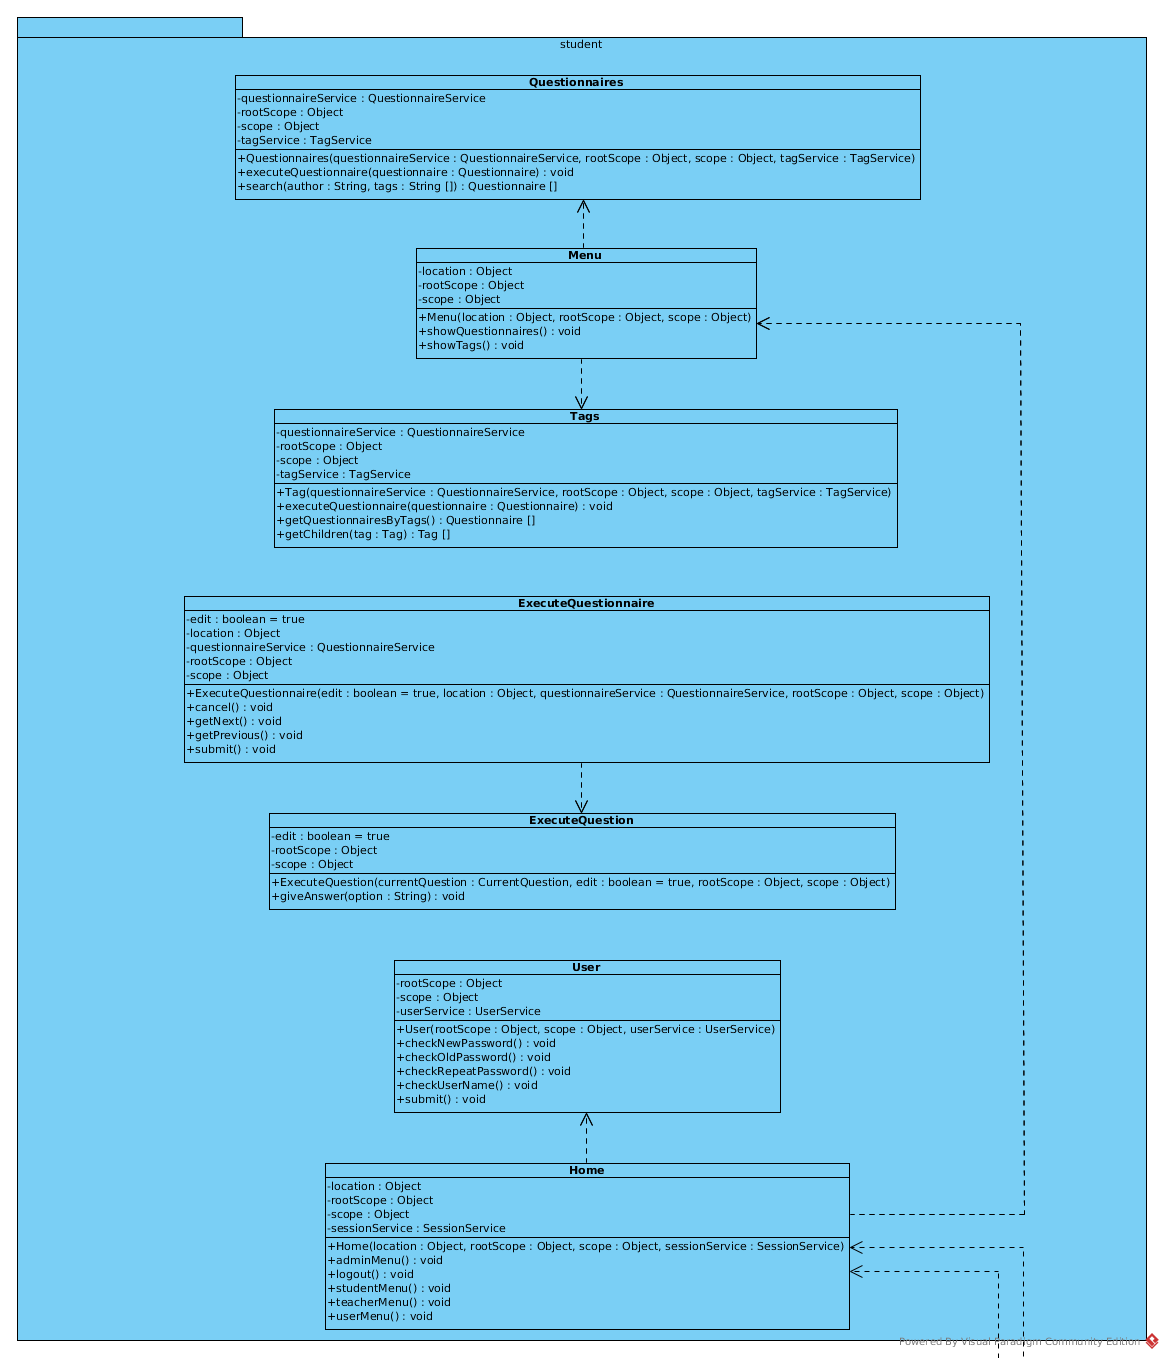
\includegraphics[scale=4, max width=\textwidth, max height=\myheight]{../img/diagrammiClassi/client/controller/student.png}
			\caption{Diagramma package - client::controller::student}
		\end{figure}
	\end{center}\hypertarget{client::controller::student::Home}{}
\subsubsubsection[Home]{client::controller::student::Home}
\begin{center}
			\begin{figure}[H]
				\centering 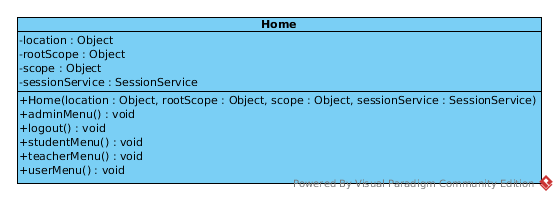
\includegraphics[scale=4, max width=\textwidth, max height=\myheight]{../img/diagrammiClassi/client/controller/student/Home.png}
				\caption{Diagramma classe - client::controller::student::Home}
			\end{figure}
		\end{center}\begin{description}
\item[Descrizione] \hfill \\
 Classe che si occupa della gestione della home page di uno studente
\item[Utilizzo] \hfill \\
 Viene richiamata dopo il login e mostra una pagina di benvenuto e la dashboard per navigare nell'applicazione
\item[Attributi] \hfill \\
 \vspace{-7mm}
\begin{itemize}
\item location : Object (analizza l'URL nella barra degli indirizzi del browser e lo rende disponibile all'applicazione)
\item scope : Object (oggetto che fa riferimento ad una porzione di model di pertinenza di questo specifico controller)
\item rootScope : Object (oggetto identificato dall’elemento con attributo ng-app)
\item sessionService : SessionService (controlla se un utente ha già una sessione attiva)
\end{itemize}

\item[Metodi] \hfill \\
 \vspace{-7mm}
\begin{itemize}
\item Home(sessionService : client.service.SessionService, location : Object, rootScope : Object, scope : Object) (costruttore della classe)\begin{itemize}
\item sessionService (Contiene il riferimento verso il servizio di sessione )
\item location (oggetto fornito da angularjs che analizza l'URL nella barra degli indirizzi del browser e lo rende disponibile all'applicazione)
\item rootScope (oggetto identificato dall’elemento con attributo ng-app)
\item scope (oggetto che fa riferimento ad una porzione di model di pertinenza di questo specifico controller)
\end{itemize}

\item adminMenu() : void (permette di aggiungere, se necessario per la tipologia di profilo autenticato, il menù lato amministratore)
\item logout() : void (chiude la sessione dello studente)
\item studentMenu() : void (gestisce il menu lato studente)
\item teacherMenu() : void (permette di aggiungere, se necessario per la tipologia di profilo autenticato, il menù lato docente)
\item userMenu() : void (gestisce il menu di primo livello dell'applicazione, per l'eventuale navigazione tra le funzionalità di ogni tipologia di profilo)
\end{itemize}

\end{description}

\vspace{0.5cm}
\hypertarget{client::controller::student::Questionnaires}{}
\subsubsubsection[Questionnaires]{client::controller::student::Questionnaires}
\begin{center}
			\begin{figure}[H]
				\centering 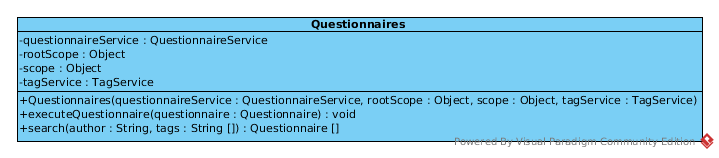
\includegraphics[scale=4, max width=\textwidth, max height=\myheight]{../img/diagrammiClassi/client/controller/student/Questionnaires.png}
				\caption{Diagramma classe - client::controller::student::Questionnaires}
			\end{figure}
		\end{center}\begin{description}
\item[Descrizione] \hfill \\
 Classe che si occupa della ricerca di un questionario da parte di uno studente e dell'eventuale gestione di una richiesta di esecuzione di un questionario
\item[Utilizzo] \hfill \\
 Si occupa di gestire la ricerca di un questionario e di permettere ad uno studente di navigare tra i questionari presenti nel sistema per sceglierne eventualmente uno da eseguire
\item[Relazioni con altre classi] \hfill \\
 \vspace{-7mm}
\begin{description}
\item[\hyperlink{client::model::data::Questionnaire}{client::model::data::Questionnaire}] \hfill \\
 Relazione uscente, lista di questionari
\item[\hyperlink{client::model::data::Tag}{client::model::data::Tag}] \hfill \\
 Relazione uscente, lista degli argomenti trattati in un questionario
\end{description}

\item[Attributi] \hfill \\
 \vspace{-7mm}
\begin{itemize}
\item rootScope : Object (oggetto identificato dall’elemento con attributo ng-app)
\item scope : Object (oggetto che fa riferimento ad una porzione di model di pertinenza di questo specifico controller)
\item tags : Tag[] (lista degli argomenti trattati in un questionario)
\item questionnaireService : QuestionnaireService (permette di creare, visualizzare, modificare e cancellare un questionario )
\item tagService : TagService (servizio che permette di creare, visualizzare, modificare e cancellare un argomento)
\item questionnaires  : Questionnaire[] (lista di questionari)
\end{itemize}

\item[Metodi] \hfill \\
 \vspace{-7mm}
\begin{itemize}
\item Questionnaires(questionnaireService : client.model.service .QuestionnaireService, rootScope : Object, scope : Object, tagService : client.model.service .TagService) (costruttore della classe)\begin{itemize}
\item questionnaireService (Contiene il riferimento verso il servizio di gestione dei questionari )
\item rootScope (oggetto identificato dall’elemento con attributo ng-app)
\item scope (oggetto che fa riferimento ad una porzione di model di pertinenza di questo specifico controller)
\item tagService (Contiene il riferimento verso il servizio di gestione degli argomenti )
\end{itemize}

\item executeQuestionnaire(questionnaire : Questionnaire) : void (permette di eseguire il questionario passato come parametro)\begin{itemize}
\item questionnaire (Contiene il questionario da eseguire)
\end{itemize}

\item search(author : String, tags  : String[]) : Questionnaire[] (permette di ricercare questionari in base ad autore e ad argomenti)\begin{itemize}
\item author (Contiene il nome dell'autore per ricercare il questionario )
\item tags  (Contiene la lista degli argomenti per ricercare il questionario )
\end{itemize}

\end{itemize}

\end{description}

\vspace{0.5cm}
\hypertarget{client::controller::student::Menu}{}
\subsubsubsection[Menu]{client::controller::student::Menu}
\begin{center}
			\begin{figure}[H]
				\centering \includegraphics[scale=4, max width=\textwidth, max height=\myheight]{../img/diagrammiClassi/client/controller/student/Menu.png}
				\caption{Diagramma classe - client::controller::student::Menu}
			\end{figure}
		\end{center}\begin{description}
\item[Descrizione] \hfill \\
 È la classe che si occupa di gestire le azioni che uno studente può compiere
\item[Utilizzo] \hfill \\
 Si occupa di mandare lo studente alle pagine dedicate alla scelta di un questionario piuttosto che di un argomento 
\item[Attributi] \hfill \\
 \vspace{-7mm}
\begin{itemize}
\item location : Object (analizza l'URL nella barra degli indirizzi del browser e lo rende disponibile all'applicazione)
\item rootScope : Object (oggetto identificato dall’elemento con attributo ng-app)
\item scope : Object (oggetto che fa riferimento ad una porzione di model di pertinenza di questo specifico controller)
\end{itemize}

\item[Metodi] \hfill \\
 \vspace{-7mm}
\begin{itemize}
\item Menu(location : Object, scope : Object, rootScope : Object) (costruttore della classe)\begin{itemize}
\item location (oggetto fornito da angularjs che analizza l'URL nella barra degli indirizzi del browser e lo rende disponibile all'applicazione)
\item scope (oggetto che fa riferimento ad una porzione di model di pertinenza di questo specifico controller)
\item rootScope (oggetto identificato dall’elemento con attributo ng-app)
\end{itemize}

\item showQuestionnaires() : void (Consente ad uno studente di entrare nella pagina preposta alla navigazione tra i questionari presenti nel sistema)
\item showTags() : void (Consente ad uno studente di accedere alla pagina preposta alla navigazione tra i tag presenti nel sistema )
\end{itemize}

\end{description}

\vspace{0.5cm}
\hypertarget{client::controller::student::Tags}{}
\subsubsubsection[Tags]{client::controller::student::Tags}
\begin{center}
			\begin{figure}[H]
				\centering \includegraphics[scale=4, max width=\textwidth, max height=\myheight]{../img/diagrammiClassi/client/controller/student/Tags.png}
				\caption{Diagramma classe - client::controller::student::Tags}
			\end{figure}
		\end{center}\begin{description}
\item[Descrizione] \hfill \\
 Classe che si occupa della gestione dell'esecuzione e della ricerca di  un questionario per argomento da parte di uno studente.
\item[Utilizzo] \hfill \\
 Si occupa dopo aver ricercato un questionario per argomento, di visualizzare le domande, raccogliere le risposte ed inviare le risposte al server.
\item[Relazioni con altre classi] \hfill \\
 \vspace{-7mm}
\begin{description}
\item[\hyperlink{client::model::data::Tag}{client::model::data::Tag}] \hfill \\
 Relazione uscente, lista di argomenti visti come un cammino che parte dalla radice fino al figlio selezionato
\item[\hyperlink{client::model::data::Questionnaire}{client::model::data::Questionnaire}] \hfill \\
 Relazione uscente, lista di questionari
\end{description}

\item[Attributi] \hfill \\
 \vspace{-7mm}
\begin{itemize}
\item rootScope : Object (oggetto identificato dall’elemento con attributo ng-app)
\item scope : Object (oggetto che fa riferimento ad una porzione di model di pertinenza di questo specifico controller)
\item questionnaireService : QuestionnaireService (servizio che ci permette di creare, visualizzare, modificare e cancellare un questionario )
\item tagService : TagService (servizio che ci permette di creare, visualizzare, modificare e cancellare un argomento)
\item path : Tag[] (lista di argomenti visti come un cammino che parte dalla radice fino al figlio selezionato)
\item questionnaires  : Questionnaire[] (lista di questionari)
\end{itemize}

\item[Metodi] \hfill \\
 \vspace{-7mm}
\begin{itemize}
\item Tags(questionnaireService : client.model.service .QuestionnaireService, rootScope : Object, scope : Object, tagService : client.model.service .TagService) (costruttore della classe)\begin{itemize}
\item questionnaireService (Contiene il riferimento verso il servizio di gestione dei questionari )
\item rootScope (oggetto identificato dall’elemento con attributo ng-app)
\item scope (oggetto che fa riferimento ad una porzione di model di pertinenza di questo specifico controller)
\item tagService (Contiene il riferimento verso il servizio di gestione degli argomenti )
\end{itemize}

\item executeQuestionnaire(questionnaire : Questionnaire) : void (permette di eseguire il questionario passato per parametro)\begin{itemize}
\item questionnaire (Contiene il questionario da eseguire)
\end{itemize}

\item getQuestionnaireByTags() : Questionnaire[] (restituisce questionari in base all'argomento )
\item getChildren(tag : Tag) : Tag[] (restituisce i figli dell'argomento passato per parametro)\begin{itemize}
\item tag (Contiene l'argomento di cui bisogna ritornare i figli )
\end{itemize}

\end{itemize}

\end{description}

\vspace{0.5cm}
\hypertarget{client::controller::student::ExecuteQuestionnaire}{}
\subsubsubsection[ExecuteQuestionnaire]{client::controller::student::ExecuteQuestionnaire}
\begin{center}
			\begin{figure}[H]
				\centering \includegraphics[scale=4, max width=\textwidth, max height=\myheight]{../img/diagrammiClassi/client/controller/student/ExecuteQuestionnaire.png}
				\caption{Diagramma classe - client::controller::student::ExecuteQuestionnaire}
			\end{figure}
		\end{center}\begin{description}
\item[Descrizione] \hfill \\
 La classe che controlla esecuzione del questionario 
\item[Utilizzo] \hfill \\
 Viene chiamata quando uno studente comincia a rispondere ad un questionario. Lo studente non è obbligato a rispondere alle domande una dopo l'altra, ha la possibilità di poter tornare su domande che in precedenza non aveva risposto. Solo dopo il submit che il questionario si considera completato
\item[Relazioni con altre classi] \hfill \\
 \vspace{-7mm}
\begin{description}
\item[\hyperlink{client::model::util::CurrentQuestionnaire}{client::model::util::CurrentQuestionnaire}] \hfill \\
 Relazione uscente, istanza del questionario di esecuzione
\end{description}

\item[Attributi] \hfill \\
 \vspace{-7mm}
\begin{itemize}
\item edit : boolean (flag booleano settato a true che controlla se il questionario è stato editato)
\item location : Object (analizza l'URL nella barra degli indirizzi del browser e lo rende disponibile all'applicazione)
\item questionnaireService : QuestionnaireService (servizio che permette di creare, visualizzare, modificare e cancellare un questionario)
\item rootScope : Object (oggetto identificato dall’elemento con attributo ng-app)
\item scope : Object (oggetto che fa riferimento ad una porzione di model di pertinenza di questo specifico controller)
\item currentQuestionnaire : CurrentQuestionnaire (istanza del questionario di esecuzione)
\end{itemize}

\item[Metodi] \hfill \\
 \vspace{-7mm}
\begin{itemize}
\item ExecuteQuestionnaire(location : Object, questionnaireService : client.service .QuestionnaireService, rootScope : Object, scope : Object, edit : boolean) (costruttore della classe)\begin{itemize}
\item location (oggetto fornito da angularjs che analizza l'URL nella barra degli indirizzi del browser e lo rende disponibile all'applicazione)
\item questionnaireService (Contiene il riferimento verso il servizio di gestione dei questionari )
\item rootScope (oggetto identificato dall’elemento con attributo ng-app)
\item scope (oggetto che fa riferimento ad una porzione di model di pertinenza di questo specifico controller)
\item edit (Indica se esecuzione del questionario è in modalità read-only. Ovvero se variabile è true allora si possono cambiare le risposte alle domande, altrimenti si può solo visualizzare il questionario senza poter cambiare le risposte già selezionate )
\end{itemize}

\item cancel() : void (permette di uscire dal currentQuestionnaire)
\item getNext() : void (va alla prossima domanda)
\item getPrevious() : void (va alla domanda precedente)
\item submit() : void (invia le risposte del currentQuestionnaire al servizio preposto)
\end{itemize}

\end{description}

\vspace{0.5cm}
\hypertarget{client::controller::student::ExecuteQuestion}{}
\subsubsubsection[ExecuteQuestion]{client::controller::student::ExecuteQuestion}
\begin{center}
			\begin{figure}[H]
				\centering \includegraphics[scale=4, max width=\textwidth, max height=\myheight]{../img/diagrammiClassi/client/controller/student/ExecuteQuestion.png}
				\caption{Diagramma classe - client::controller::student::ExecuteQuestion}
			\end{figure}
		\end{center}\begin{description}
\item[Descrizione] \hfill \\
 La classe che controlla l'esecuzione di una domanda 
\item[Utilizzo] \hfill \\
 Viene chiamata per dare la possibilità ad uno studente di eseguire una specifica domanda all'interno di un questionario in esecuzione
\item[Relazioni con altre classi] \hfill \\
 \vspace{-7mm}
\begin{description}
\item[\hyperlink{client::model::util::CurrentQuestion}{client::model::util::CurrentQuestion}] \hfill \\
 Relazione uscente, domanda corrente
\end{description}

\item[Attributi] \hfill \\
 \vspace{-7mm}
\begin{itemize}
\item edit : boolean (lag booleano settato a true che controlla se la domanda ha ricevuto una risposta o no)
\item rootScope : Object (oggetto identificato dall’elemento con attributo ng-app)
\item scope : Object (oggetto che fa riferimento ad una porzione di model di pertinenza di questo specifico controller)
\item currentQuestion : CurrentQuestion  (domanda corrente)
\end{itemize}

\item[Metodi] \hfill \\
 \vspace{-7mm}
\begin{itemize}
\item ExecuteQuestion(currentQuestion : client.model.util.CurrentQuestion, edit : boolean, rootScope : Object, scope : Object) (costruttore della classe)\begin{itemize}
\item currentQuestion (Contiene la domanda corrente da eseguire )
\item edit (True - si può modificare, false - no )
\item rootScope (oggetto identificato dall’elemento con attributo ng-app)
\item scope (oggetto che fa riferimento ad una porzione di model di pertinenza di questo specifico controller)
\end{itemize}

\item giveAnswer(option : String) : void (inserisce la risposta option nella domanda corrente)\begin{itemize}
\item option (Contiene la risposta alla domanda  data dall'utente )
\end{itemize}

\end{itemize}

\end{description}

\vspace{0.5cm}
\hypertarget{client::controller::student::User}{}
\subsubsubsection[User]{client::controller::student::User}
\begin{center}
			\begin{figure}[H]
				\centering \includegraphics[scale=4, max width=\textwidth, max height=\myheight]{../img/diagrammiClassi/client/controller/student/User.png}
				\caption{Diagramma classe - client::controller::student::User}
			\end{figure}
		\end{center}\begin{description}
\item[Descrizione] \hfill \\
 Classe per la gestione del profilo di uno studente
\item[Utilizzo] \hfill \\
 Si occupa della gestione delle informazioni del profilo di uno studente e fornisce le funzionalità di modifica di queste ultime, controllando opportunamente i valori inseriti
\item[Relazioni con altre classi] \hfill \\
 \vspace{-7mm}
\begin{description}
\item[\hyperlink{client::model::data::User}{client::model::data::User}] \hfill \\
 Relazione uscente, utente loggato
\end{description}

\item[Attributi] \hfill \\
 \vspace{-7mm}
\begin{itemize}
\item scope : Object (oggetto che fa riferimento ad una porzione di model di pertinenza di questo specifico controller)
\item rootScope : Object (oggetto identificato dall’elemento con attributo ng-app)
\item userService : UserService (si occupa della operazioni di inserimento, modifica e rimozione di account utente)
\item me : User  (utente loggato)
\end{itemize}

\item[Metodi] \hfill \\
 \vspace{-7mm}
\begin{itemize}
\item User(rootScope : Object, scope : Object, userService : client.service .UserService) (costruttore della classe)\begin{itemize}
\item rootScope (oggetto identificato dall’elemento con attributo ng-app)
\item scope (oggetto che fa riferimento ad una porzione di model di pertinenza di questo specifico controller)
\item userService (Contiene il riferimento verso il servizio di gestione degli utenti )
\end{itemize}

\item checkNewPassword() : void (controlla se la nuova password è conforme ai requisiti minimi)
\item checkOldPassword() : void (controlla se la password inserita coincide con quella attualmente in vigore)
\item checkRepeatPassword() : void (controlla se questa password coincide con la newPassword)
\item checkUserName() : void (controlla se lo userName ha i requisiti minimi)
\item submit() : void (invia i dati dello studente al servizio preposto)
\end{itemize}

\end{description}

\vspace{0.5cm}
\subsubsection{client::controller::teacher}
È il package che contiene tutte le classi che costituiscono i controller della porzione client per un docente. Ogni componente si occupa della gestione di una particolare porzione dell'interfaccia di un docente.\begin{center}
		\begin{figure}[H]
			\centering \includegraphics[scale=4, max width=\textwidth, max height=\myheight]{../img/diagrammiClassi/client/controller/teacher.png}
			\caption{Diagramma package - client::controller::teacher}
		\end{figure}
	\end{center}\hypertarget{client::controller::teacher::ManipulateTag}{}
\subsubsubsection[ManipulateTag]{client::controller::teacher::ManipulateTag}
\begin{center}
			\begin{figure}[H]
				\centering \includegraphics[scale=4, max width=\textwidth, max height=\myheight]{../img/diagrammiClassi/client/controller/teacher/ManipulateTag.png}
				\caption{Diagramma classe - client::controller::teacher::ManipulateTag}
			\end{figure}
		\end{center}\begin{description}
\item[Descrizione] \hfill \\
 Classe che si occupa della gestione della gerarchia di argomenti presenti nell'applicazione
\item[Utilizzo] \hfill \\
 Classe che aggiunge o modifica argomenti nella gerarchia di argomenti già esistente
\item[Relazioni con altre classi] \hfill \\
 \vspace{-7mm}
\begin{description}
\item[\hyperlink{client::model::data::Tag}{client::model::data::Tag}] \hfill \\
 Relazione uscente, rappresenta il nome e la descrizione di un argomento
\end{description}

\item[Attributi] \hfill \\
 \vspace{-7mm}
\begin{itemize}
\item scope : Object (oggetto che fa riferimento ad una porzione di model di pertinenza di uno specifico controller)
\item rootScope : Object (oggetto identificato dall’elemento con attributo ng-app)
\item tagService : TagService (permette di creare, visualizzare, modificare e cancellare un argomento)
\item tag  : Tag  (rappresenta il nome e la descrizione di un argomento)
\end{itemize}

\item[Metodi] \hfill \\
 \vspace{-7mm}
\begin{itemize}
\item ManipulateTag(rootScope : Object, scope : Object, tag : client.model.data.Tag, tagService : client.model.service.TagService) (costruttore della classe )\begin{itemize}
\item rootScope (oggetto identificato dall’elemento con attributo ng-app)
\item scope (oggetto che fa riferimento ad una porzione di model di pertinenza di questo specifico controller)
\item tag (Continente il riferimento verso il modello degli argomenti )
\item tagService (Contiene il riferimento verso il servizio di gestione degli argomenti )
\end{itemize}

\item setParent(parent : client.model.data.Tag) : void (imposta il tag passato come padre dell'argomento d'istanza)\begin{itemize}
\item parent (Contiene il padre dell'argomento da modificare)
\end{itemize}

\item submit() : void (invia i dati al servizio preposto)
\end{itemize}

\end{description}

\vspace{0.5cm}
\hypertarget{client::controller::teacher::ManipulateQuestion}{}
\subsubsubsection[ManipulateQuestion]{client::controller::teacher::ManipulateQuestion}
\begin{center}
			\begin{figure}[H]
				\centering \includegraphics[scale=4, max width=\textwidth, max height=\myheight]{../img/diagrammiClassi/client/controller/teacher/ManipulateQuestion.png}
				\caption{Diagramma classe - client::controller::teacher::ManipulateQuestion}
			\end{figure}
		\end{center}\begin{description}
\item[Descrizione] \hfill \\
 Classe che si occupa della gestione della domanda lato docente
\item[Utilizzo] \hfill \\
 Viene richiamata quando un docente vuole aggiungere,  modificare o eliminare una domanda
\item[Relazioni con altre classi] \hfill \\
 \vspace{-7mm}
\begin{description}
\item[\hyperlink{client::model::data::Question}{client::model::data::Question}] \hfill \\
 Relazione uscente, oggetto che rappresenta una singola domanda
\end{description}

\item[Attributi] \hfill \\
 \vspace{-7mm}
\begin{itemize}
\item question : Question  (oggetto che rappresenta una singola domanda)
\item rootScope : Object (oggetto identificato dall’elemento con attributo ng-app)
\item questionService : QuestionService (servizio che permette di creare, visualizzare, modificare e cancellare una domanda)
\item scope : Object (oggetto che fa riferimento ad una porzione di model di pertinenza di uno specifico controller)
\end{itemize}

\item[Metodi] \hfill \\
 \vspace{-7mm}
\begin{itemize}
\item ManipulateQuestion(question : client.model.data.Question, questionService : client.model.service .QuestionService, scope : Object, rootScope : Object) (costruttore della classe)\begin{itemize}
\item question (Contiene il riferimento verso il modello delle domande )
\item questionService (Contiene il riferimento verso il servizio di gestione delle domande )
\item scope (oggetto che fa riferimento ad una porzione di model di pertinenza di questo specifico controller)
\item rootScope (oggetto identificato dall’elemento con attributo ng-app)
\end{itemize}

\item addTag(tag : Tag) : void (aggiunge l'argomento passato come parametro alla domanda corrente)\begin{itemize}
\item tag (Contiene l'argomento da aggiungere alla domanda)
\end{itemize}

\item removeTag(tag : Tag) : void (elimina l'argomento passato come parametro da quelli della domanda corrente)\begin{itemize}
\item tag (Contiene l'argomento da eliminare dalla lista degli argomenti della domanda)
\end{itemize}

\item submit() : void (invia i dati al servizio preposto)
\end{itemize}

\end{description}

\vspace{0.5cm}
\hypertarget{client::controller::teacher::ManipulateQuestionnaire}{}
\subsubsubsection[ManipulateQuestionnaire]{client::controller::teacher::ManipulateQuestionnaire}
\begin{center}
			\begin{figure}[H]
				\centering \includegraphics[scale=4, max width=\textwidth, max height=\myheight]{../img/diagrammiClassi/client/controller/teacher/ManipulateQuestionnaire.png}
				\caption{Diagramma classe - client::controller::teacher::ManipulateQuestionnaire}
			\end{figure}
		\end{center}\begin{description}
\item[Descrizione] \hfill \\
 Classe che si occupa della gestione di un questionario lato docente
\item[Utilizzo] \hfill \\
 Viene richiamata quando un docente vuole creare un nuovo questionario o modificare o eliminare uno già esistente
\item[Relazioni con altre classi] \hfill \\
 \vspace{-7mm}
\begin{description}
\item[\hyperlink{client::model::data::Questionnaire}{client::model::data::Questionnaire}] \hfill \\
 Relazione uscente, oggetto che rappresenta un questionario
\end{description}

\item[Attributi] \hfill \\
 \vspace{-7mm}
\begin{itemize}
\item questionnaire : Questionnaire (oggetto che rappresenta un questionario)
\item questionnaireService : QuestionnaireService (servizio che permette di creare, visualizzare, modificare e cancellare un questionario)
\item rootScope : Object (oggetto identificato dall’elemento con attributo ng-app)
\item scope : Object (oggetto che fa riferimento ad una porzione di model di pertinenza di uno specifico controller)
\end{itemize}

\item[Metodi] \hfill \\
 \vspace{-7mm}
\begin{itemize}
\item ManipulateQuestionnaire(questionnaireService : client.model.data.QuestionnaireService, questionnaire : client.model.data.Questionnaire, scope : Object, rootScope : Object) (costruttore della classe)\begin{itemize}
\item questionnaireService (Contiene il riferimento al servizio di gestione dei questionari )
\item questionnaire (Contiene il riferimento al modello degli questionari )
\item scope (oggetto che fa riferimento ad una porzione di model di pertinenza di questo specifico controller)
\item rootScope (oggetto identificato dall’elemento con attributo ng-app)
\end{itemize}

\item addQuestion(question : Question) : void (aggiunge la domanda passata come parametro al questionario d'istanza)\begin{itemize}
\item question (Contiene la domanda da aggiungere al questionario )
\end{itemize}

\item addTag(tag : Tag) : void (aggiunge l'argomento passato come parametro a quelli del questionario corrente)\begin{itemize}
\item tag (Contiene l'argomento da aggiungere alla lista degli argomenti del questionario  )
\end{itemize}

\item removeTag(tag : Tag) : void (rimuove l'argomento passato come parametro da quelli assegnati al questionario corrente)\begin{itemize}
\item tag (Contiene l'argomento da eliminare dalla lista degli argomenti del questionario )
\end{itemize}

\item removeQuestion(question : Question) : void (rimuove la domanda passata per parametro dal questionario d'istanza)\begin{itemize}
\item question (Contiene la domanda da eliminare dal questionario )
\end{itemize}

\item selectQuestion() : void (seleziona una domanda nel questionario d'istanza)
\item submit() : void (invia il dati presenti nel questionario al servizio preposto)
\end{itemize}

\end{description}

\vspace{0.5cm}
\hypertarget{client::controller::teacher::SelectQuestion}{}
\subsubsubsection[SelectQuestion]{client::controller::teacher::SelectQuestion}
\begin{center}
			\begin{figure}[H]
				\centering \includegraphics[scale=4, max width=\textwidth, max height=\myheight]{../img/diagrammiClassi/client/controller/teacher/SelectQuestion.png}
				\caption{Diagramma classe - client::controller::teacher::SelectQuestion}
			\end{figure}
		\end{center}\begin{description}
\item[Descrizione] \hfill \\
 Classe che gestisce la ricerca di una domanda e la sua eventuale selezione
\item[Utilizzo] \hfill \\
 Viene chiamata quando in fase di costruzione di un questionario si ha la necessità di ricercare per poi inserire una particolare domanda
\item[Relazioni con altre classi] \hfill \\
 \vspace{-7mm}
\begin{description}
\item[\hyperlink{client::model::data::Tag}{client::model::data::Tag}] \hfill \\
 Relazione uscente, lista degli argomenti associati ad un questionario
\end{description}

\item[Attributi] \hfill \\
 \vspace{-7mm}
\begin{itemize}
\item questionService : QuestionService (servizio che permette di creare, visualizzare, modificare e cancellare una domanda)
\item rootScope : Object (oggetto identificato dall’elemento con attributo ng-app)
\item scope : Object (oggetto che fa riferimento ad una porzione di model di pertinenza di uno specifico controller)
\item tags  : Tag[] (lista degli argomenti associati ad un questionario)
\end{itemize}

\item[Metodi] \hfill \\
 \vspace{-7mm}
\begin{itemize}
\item SelectQuestion(questionService : QuestionService, rootScope : Object, scope : Object) (costruttore della classe)\begin{itemize}
\item questionService (Contiene il riferimento verso il servizio di gestione delle domande )
\item rootScope (oggetto identificato dall’elemento con attributo ng-app)
\item scope (oggetto che fa riferimento ad una porzione di model di pertinenza di questo specifico controller)
\end{itemize}

\item search(author : String, keywordsQuery : String) : void (trova tutte le domande correlate ad un autore e a delle parole chiave passati come parametro)\begin{itemize}
\item author (Contiene il nome dell'autore della domanda da ricercare )
\item keywordsQuery (Contiene la lista di parole chiave per ricercare la domanda)
\end{itemize}

\item selectQuestion() : Question (seleziona e restituisce una specifica  domanda)
\end{itemize}

\end{description}

\vspace{0.5cm}
\hypertarget{client::controller::teacher::Menu}{}
\subsubsubsection[Menu]{client::controller::teacher::Menu}
\begin{center}
			\begin{figure}[H]
				\centering \includegraphics[scale=4, max width=\textwidth, max height=\myheight]{../img/diagrammiClassi/client/controller/teacher/Menu.png}
				\caption{Diagramma classe - client::controller::teacher::Menu}
			\end{figure}
		\end{center}\begin{description}
\item[Descrizione] \hfill \\
 Classe che si occupa di gestire le azioni specifiche che un docente può compiere
\item[Utilizzo] \hfill \\
 Si occupa di mandare il docente alle pagine dedicate per la creazione di nuove domande, di nuovi questionari.
\item[Attributi] \hfill \\
 \vspace{-7mm}
\begin{itemize}
\item location : Object (analizza l'URL nella barra degli indirizzi del browser e lo rende disponibile all'applicazione)
\item scope : Object (oggetto che fa riferimento ad una porzione di model di pertinenza di uno specifico controller)
\item rootScope : Object (oggetto identificato dall’elemento con attributo ng-app)
\end{itemize}

\item[Metodi] \hfill \\
 \vspace{-7mm}
\begin{itemize}
\item Menu(location : Object, rootScope : Object, scope : Object) (costruttore della classe)\begin{itemize}
\item location (oggetto fornito da angularjs che analizza l'URL nella barra degli indirizzi del browser e lo rende disponibile all'applicazione)
\item rootScope (oggetto identificato dall’elemento con attributo ng-app)
\item scope (oggetto che fa riferimento ad una porzione di model di pertinenza di questo specifico controller)
\end{itemize}

\item newQuestionnaire() : void (crea un nuovo questionario)
\item newQuestion () : void (crea una nuova domanda)
\item newTag() : void (crea un nuovo argomento)
\item showQuestionnaires() : void (mostra tutti i questionari creati dal docente autenticato)
\item showQuestions() : void (mostra tutte le domande create dal docente autenticato)
\item showTags() : void (mostra tutti gli argomenti creati dal docente autenticato)
\end{itemize}

\end{description}

\vspace{0.5cm}
\hypertarget{client::controller::teacher::ManageTags}{}
\subsubsubsection[ManageTags]{client::controller::teacher::ManageTags}
\begin{center}
			\begin{figure}[H]
				\centering \includegraphics[scale=4, max width=\textwidth, max height=\myheight]{../img/diagrammiClassi/client/controller/teacher/ManageTags.png}
				\caption{Diagramma classe - client::controller::teacher::ManageTags}
			\end{figure}
		\end{center}\begin{description}
\item[Descrizione] \hfill \\
 Classe che si occupa della gestione degli argomenti lato docente
\item[Utilizzo] \hfill \\
 Viene richiamata quando un docente vuole creare un nuovo argomento o modificarne o eliminarne uno già esistente
\item[Relazioni con altre classi] \hfill \\
 \vspace{-7mm}
\begin{description}
\item[\hyperlink{client::model::data::Tag}{client::model::data::Tag}] \hfill \\
 Relazione uscente, lista di argomenti visti come un cammino che parte dalla radice fino al figlio selezionato
\end{description}

\item[Attributi] \hfill \\
 \vspace{-7mm}
\begin{itemize}
\item path : Tag[] (lista di argomenti visti come un cammino che parte dalla radice fino al figlio selezionato)
\item scope : Object (oggetto che fa riferimento ad una porzione di model di pertinenza di uno specifico controller)
\item tagService : TagService (si occupa della operazioni di inserimento, modifica e rimozione di un argomento)
\item rootScope : Object (oggetto identificato dall’elemento con attributo ng-app)
\end{itemize}

\item[Metodi] \hfill \\
 \vspace{-7mm}
\begin{itemize}
\item ManageTags(rootScope : Object, scope : Object, tagService : client.model.service .TagService) (costruttore della classe)\begin{itemize}
\item rootScope (oggetto identificato dall’elemento con attributo ng-app)
\item scope (oggetto che fa riferimento ad una porzione di model di pertinenza di questo specifico controller)
\item tagService (Contiene il riferimento al servizio di gestione degli argomenti )
\end{itemize}

\item getChildren(tag : Tag) : Tag[] (restituisce tutti i figli dell'argomento passato come parametro)\begin{itemize}
\item tag (Contiene l'argomento per cui bisogna ritornare i propri figli )
\end{itemize}

\item new() : void (crea un nuovo argomento)
\item modify(tag : Tag) : void (modifica l'argomento passato per parametro)\begin{itemize}
\item tag (Contiene l'argomento che serve modificare )
\end{itemize}

\item remove (tag : Tag) : void (rimuove l'argomento passato per argomento)\begin{itemize}
\item tag (Contiene l'argomento da eliminare )
\end{itemize}

\end{itemize}

\end{description}

\vspace{0.5cm}
\hypertarget{client::controller::teacher::ManageQuestions}{}
\subsubsubsection[ManageQuestions]{client::controller::teacher::ManageQuestions}
\begin{center}
			\begin{figure}[H]
				\centering \includegraphics[scale=4, max width=\textwidth, max height=\myheight]{../img/diagrammiClassi/client/controller/teacher/ManageQuestions.png}
				\caption{Diagramma classe - client::controller::teacher::ManageQuestions}
			\end{figure}
		\end{center}\begin{description}
\item[Descrizione] \hfill \\
 La classe che controlla la gestione delle domande create dal docente autenticato
\item[Utilizzo] \hfill \\
 Viene richiamata quando un docente vuole creare un nuova domanda o modificarne o eliminarne una già esistente tra quelle da lui create
\item[Relazioni con altre classi] \hfill \\
 \vspace{-7mm}
\begin{description}
\item[\hyperlink{client::model::data::Question}{client::model::data::Question}] \hfill \\
 Relazione uscente, lista delle domande create da uno stesso docente
\end{description}

\item[Attributi] \hfill \\
 \vspace{-7mm}
\begin{itemize}
\item scope : Object (oggetto che fa riferimento ad una porzione di model di pertinenza di uno specifico controller)
\item rootScope : Object (oggetto identificato dall’elemento con attributo ng-app)
\item questionService : QuestionService (servizio che permette di creare, visualizzare, modificare e cancellare una domanda)
\item questions  : Question[] (lista delle domande create da uno stesso docente)
\end{itemize}

\item[Metodi] \hfill \\
 \vspace{-7mm}
\begin{itemize}
\item ManageQuestions(questionnaireService : client.model.service .QuestionService, scope : Object, rootScope : Object) (costruttore della classe)\begin{itemize}
\item questionnaireService (Contiene il riferimento verso il servizio di gestione delle domande  )
\item scope (oggetto che fa riferimento ad una porzione di model di pertinenza di questo specifico controller)
\item rootScope (oggetto identificato dall’elemento con attributo ng-app)
\end{itemize}

\item new() : void (crea una nuova domanda)
\item modify(question : Question) : void (modifica la domanda passata per parametro)\begin{itemize}
\item question (Contiene  la domanda da modificare )
\end{itemize}

\item remove (question : Question) : void (elimina la domanda passata per parametro)\begin{itemize}
\item question (Contiene la domanda da eliminare )
\end{itemize}

\end{itemize}

\end{description}

\vspace{0.5cm}
\hypertarget{client::controller::teacher::ManageQuestionnaires}{}
\subsubsubsection[ManageQuestionnaires]{client::controller::teacher::ManageQuestionnaires}
\begin{center}
			\begin{figure}[H]
				\centering \includegraphics[scale=4, max width=\textwidth, max height=\myheight]{../img/diagrammiClassi/client/controller/teacher/ManageQuestionnaires.png}
				\caption{Diagramma classe - client::controller::teacher::ManageQuestionnaires}
			\end{figure}
		\end{center}\begin{description}
\item[Descrizione] \hfill \\
 La classe che controlla la gestione dei questionari creati dal docente autenticato
\item[Utilizzo] \hfill \\
 Viene richiamata quando un docente vuole creare un nuovo questionario o modificarne o eliminarne uno già esistente tra quelli da lui crearti
\item[Relazioni con altre classi] \hfill \\
 \vspace{-7mm}
\begin{description}
\item[\hyperlink{client::model::data::Questionnaire}{client::model::data::Questionnaire}] \hfill \\
 Relazione uscente, lista di questionari
\end{description}

\item[Attributi] \hfill \\
 \vspace{-7mm}
\begin{itemize}
\item scope : Object (oggetto che fa riferimento ad una porzione di model di pertinenza di questo specifico controller)
\item rootScope : Object (oggetto identificato dall’elemento con attributo ng-app)
\item questionnaireService : QuestionnaireService (servizio che permette di creare, visualizzare, modificare e cancellare un questionario)
\item questionnaires  : Questionnaire[] (lista di questionari)
\end{itemize}

\item[Metodi] \hfill \\
 \vspace{-7mm}
\begin{itemize}
\item ManageQuestionnaires(questionnaireService : client.model.service .QuestionnaireService, scope : Object, rootScope : Object) (costruttore della classe)\begin{itemize}
\item questionnaireService (Contiene il riferimento verso il servizio di  gestione dei questionari )
\item scope (oggetto che fa riferimento ad una porzione di model di pertinenza di questo specifico controller)
\item rootScope (oggetto identificato dall’elemento con attributo ng-app)
\end{itemize}

\item new() : void (crea un nuovo questionario)
\item modify(questionnaire : Questionnaire) : void (modifica il questionario passato come parametro)\begin{itemize}
\item questionnaire (Contiene il questionario da modificare )
\end{itemize}

\item remove (questionnaire : Questionnaire) : void (elimina il questionario passato come parametro)\begin{itemize}
\item questionnaire ( Contiene il questionario da eliminare )
\end{itemize}

\end{itemize}

\end{description}

\vspace{0.5cm}
\subsubsection{client::controller::admin}
È il package che contiene tutte le classi che costituiscono i controller della porzione client per un amministratore. Ogni componente si occupa della gestione di una particolare porzione dell'interfaccia di un amministratore.\begin{center}
		\begin{figure}[H]
			\centering \includegraphics[scale=4, max width=\textwidth, max height=\myheight]{../img/diagrammiClassi/client/controller/admin.png}
			\caption{Diagramma package - client::controller::admin}
		\end{figure}
	\end{center}\hypertarget{client::controller::admin::UsersList}{}
\subsubsubsection[UsersList]{client::controller::admin::UsersList}
\begin{center}
			\begin{figure}[H]
				\centering \includegraphics[scale=4, max width=\textwidth, max height=\myheight]{../img/diagrammiClassi/client/controller/admin/UsersList.png}
				\caption{Diagramma classe - client::controller::admin::UsersList}
			\end{figure}
		\end{center}\begin{description}
\item[Descrizione] \hfill \\
 Classe che si occupa della gestione di tutti gli utenti presenti nell'applicazione. In particolare gestisce l'eventuale cambio di ruolo di un utente e la sua rimozione dal sistema.
\item[Utilizzo] \hfill \\
 Carica la view che permette avere la lista completa dei tutti gli utenti, consentendo di selezionare l'utente per modificarne il ruolo o per rimuoverlo dal sistema
\item[Relazioni con altre classi] \hfill \\
 \vspace{-7mm}
\begin{description}
\item[\hyperlink{client::model::data::User}{client::model::data::User}] \hfill \\
 Relazione uscente, lista di utenti
\end{description}

\item[Attributi] \hfill \\
 \vspace{-7mm}
\begin{itemize}
\item scope : Object (oggetto che fa riferimento ad una porzione di model di pertinenza di questo specifico controller)
\item rootScope : Object (oggetto identificato dall’elemento con attributo ng-app)
\item userService : UserService (si occupa della operazioni di modifica e rimozione di account utente)
\item roleService : RoleService (permette di creare, visualizzare, modificare e cancellare il ruolo che un utente può avere)
\item usersList : User[] (lista di utenti)
\end{itemize}

\item[Metodi] \hfill \\
 \vspace{-7mm}
\begin{itemize}
\item UsersList(scope : Object, roleService : client.model.service .RoleService, rootScope : Object, userService : client.service .UserService) (costruttore della classe)\begin{itemize}
\item scope (oggetto che fa riferimento ad una porzione di model di pertinenza di questo specifico controller)
\item roleService (Contiene il riferimento verso il servizio di gestione dei ruoli )
\item rootScope (oggetto identificato dall’elemento con attributo ng-app)
\item userService (Contiene il riferimento verso il servizio di gestione degli utenti )
\end{itemize}

\item changeUserRole(user  : User, role  : client.model.data.Role) : void (cambia il ruolo di un utente )\begin{itemize}
\item user  (Contiene l'utente a cui serve cambiare il ruolo)
\item role  (Contiene il nuovo ruolo dell'utente )
\end{itemize}

\item deleteUser(user  : User) : void (elimina l'utente passato per parametro)\begin{itemize}
\item user  (Contiene l'utente da eliminare )
\end{itemize}

\end{itemize}

\end{description}

\vspace{0.5cm}
\hypertarget{client::controller::admin::Menu}{}
\subsubsubsection[Menu]{client::controller::admin::Menu}
\begin{center}
			\begin{figure}[H]
				\centering \includegraphics[scale=4, max width=\textwidth, max height=\myheight]{../img/diagrammiClassi/client/controller/admin/Menu.png}
				\caption{Diagramma classe - client::controller::admin::Menu}
			\end{figure}
		\end{center}\begin{description}
\item[Descrizione] \hfill \\
 Questa classe gestisce la visualizzazione di tutti gli utenti del sistema.
\item[Utilizzo] \hfill \\
 Viene chiamata quando un amministratore vuole osservare una porzione di tutti gli utenti presenti nel database in base al ruolo che si è scelto.
\item[Attributi] \hfill \\
 \vspace{-7mm}
\begin{itemize}
\item location : Object (analizza l'URL nella barra degli indirizzi del browser e lo rende disponibile all'applicazione)
\item scope : Object (oggetto che fa riferimento ad una porzione di model di pertinenza di questo specifico controller)
\item rootScope : Object (oggetto identificato dall’elemento con attributo ng-app)
\end{itemize}

\item[Metodi] \hfill \\
 \vspace{-7mm}
\begin{itemize}
\item Menu(location : Object, rootScope : Object, scope : Object) (costruttore della classe)\begin{itemize}
\item location (oggetto fornito da angularjs che analizza l'URL nella barra degli indirizzi del browser e lo rende disponibile all'applicazione)
\item rootScope (oggetto identificato dall’elemento con attributo ng-app)
\item scope (oggetto che fa riferimento ad una porzione di model di pertinenza di questo specifico controller)
\end{itemize}

\item showAdmins() : void (mostra tutti gli amministratori)
\item showStudents() : void (mostra tutti gli studenti)
\item showTeachers() : void (mostra tutti i docenti)
\end{itemize}

\end{description}

\vspace{0.5cm}
